%%% -*-LaTeX-*-

\chapter{Automated Concurrency Testing Framework for Go}
\label{sec:ch4}

This chapter is based on the work submitted to the 2021 IEEE International Symposium on Workload Characterization (IISWC).
We present \goat, a combined static and dynamic concurrency testing
and analysis tool that facilitate the process of debugging for real-world programs.
%
Key ideas in \goat include
1) automated dynamic tracing to capture the behavior of concurrency primitives,
2) systematic schedule space exploration to accelerate the bug occurance
and 3) deadlock detection with supplementary visualizations and reports.
We also propose a set of coverage requirements that characeterize the dynamic behavior of concurrency primitives and provide metrics to measure the quality of tests.
%
Our evaluation on 68 curated real-world bug scenarios
demonstrates that GoAT is significantly effective in detecting
rare bugs, and its schedule perturbation method based on schedule
yielding detects these bugs with less than three yields.
%
These results together with the ease of deploying GoAT on real-world
Go programs holds significant promise in field-debugging of Go programs.

\section{Introduction}
\label{sec:ch4_intro}
Go~\cite{go} is a statically typed language initially developed by Google.
%
It employs channel-based Hoare's Communicating Sequential Processes (CSP)~\cite{hoare-csp78} semantics in its core and provides a productivity-enhancing environment for concurrent programming.
%
Go enjoys accelerating acceptance in a wide variety of
communities including container software systems~\cite{merkel2014docker,kubernetes},  distributed key-value databases~\cite{etcd,cockroachdb-sigmod20}, and web server libraries \cite{grpc}.
%
It involves shared memory, message passing, nondeterministic message reception and selection, dynamic process creation, and programming styles that tend to create thousands of \textit{goroutines}~(\ie,~application-level threads) and discard them to be garbage collected when they reach their final state.
%
The combination of these features is well known for Go's popularity, yet they also make Go challenging to debug.
%
Our work is especially relevant considering that there are no widely practical tools for debugging concurrent Go; even well-curated
concurrency bug benchmark suites are only just now beginning to appear~\cite{tu-concurrentBugs-asplos19,yuan-gobench-cgo21}.
%

In general, concurrent bugs are notoriously difficult to find and reproduce due to the nondeterministic choices that the scheduler makes during execution.
%
In Go, constructs like \textit{select} and buffered channels entangle the process of debugging by introducing extra randomness to the dynamic behavior of the program.
%
Recent static~\cite{ng-dl-cc16,stadtmuller-minigo-aplas16,lange-fence-popl17,lange-staticType-icse18} and dynamic~\cite{go-race-blog,zhao-occam97,sulzmann-corr17,sulzmann-twophase-2018,dilley-gomela-corr2020} techniques have been proposed to address these challenges.
%
GoBench \cite{yuan-gobench-cgo21} gathers a collection of real concurrency bugs (GoReal) and simplified bug kernels (GoKer) from top 9 open-source projects written in Go and evaluated the effectivness such techniques in detecting the bug collection.
%
Although static methods are proved to be rigorously effective in detecting flaws in small programs, they are not practical for realistic programs and often produce false positives.
%
On the other hand, dynamic analysis approaches cover a more significant subset of real-world programs by constructing and analyzing an \textit{execution model}.
%
However, they focus on a specific class of bugs based on the symptom or cause of the bug.
%
Also, for large codebases with thousands of LOC, it is nontrivial to capture an accurate dynamic execution model using source instrumentation or source-to-source translation.
%
Furthermore, our experiments (Section \ref{sec:ch4_evaluation}) observe that some buggy programs take more than 1,000 runs under different schedules before the bug is hit.
%
Concurrent testing methods~\cite{arora-concrrentTesting-16} are proposed to complement static and dynamic approaches in tackling challenges of concurrent debugging.
%
To the best of our knowledge, there exist no such testing methods applicable to Go.
%




We implemented \goat (\textbf{Go} \textbf{A}nalysis and \textbf{T}esting), a debugging framework for concurrent Go applications to address this lack.
%
\goat (Figure \ref{fig:goat_workflow}) combines static and dynamic approaches to automatically analyze the behavior of concurrent components and facilitate the process of testing and debugging Go applications.
%
%We evaluated \goat and compared it against similar tools on the recent Go concurrent bug benchmark~\cite{yuan-gobench-cgo21}.
%
Several classic ideas from literature are combined with novel ones to support modern concepts of Go in \goat, which pursues three primary objectives.
\\
\subsection{Objective 1: Accurate Dynamic Execution Modeling}
In order to study the behavior of concurrent components and track the state of the program during execution, a dynamic execution model has to be constructed and compared against a predefined model (e.g., formally defined specifications or the developer's mental representation of the program).
%
It is crucial for debuggers and software analysis tools to construct their execution models as close as possible to the actual program execution context.
%
Since a bug might occur at various levels of abstraction, \textit{whole-program dynamic tracing} provides a practical and uniform way to track multiple facets of the program during execution~\cite{diffTrace}.
%
We have enhanced the built-in tracing mechanism of Go~\cite{ect-arxiv} to capture the dynamic behavior of concurrency primitives in the form of a \textit{sequence of events}, namely \textit{execution concurrency trace} or ECT.
%
Each event in ECT represents an \textit{action} that corresponds to exactly one statement in the source code.
%
An ECT provides a detailed model of how a concurrent program behaves dynamically and assists debugging procedures (e.g., bug detection, root-cause analysis, execution visualization).
%
Our experiments show that by replaying the program's ECT, \goat detects all blocking bugs of GoKer~\cite{yuan-gobench-cgo21} many of which are undetected by existing debugging tools.

\subsection{Objective 2: Systematic Exploration of Schedule-Space}
Since the scheduler's nondeterministic behavior is the primary reason for Heisenbugs (\ie, errors that are uncommon to occur and hard to reproduce), these bugs may not manifest during conventional testing.
%
By adopting ideas from \textit{systematic concurrency testing} approaches~\cite{dpor,thomson-concurrencyTesting-ppopp14,emmi-delayBounded-popl11,burckhardt-depthBug-asplos10,madanlal-preemptionBound-pldi07,yu-maple-oopsla12,joshi-calfuzzer,contest-jgi01,edelstein2003contest,hong-syncTesting-issta12,christakis-erlang-icst13,yuan-morpheus-asplos20}, we perturb the native scheduler of Go to explore the unconventional but feasible execution interleaving.
%
First, we statically identify the source location of concurrency primitive usages in a given program.
%
We then inject handlers of context-switching calls around these locations to manage schedule perturbation.
%
At its simplest form, handlers randomly (with a certain probablity and within a bound) decide if the current goroutine should continue executing or \textit{yield} to other goroutines to execute first.
%
Such yields change the blocking behavior of the program within the space of feasible states and exercise untested interleavings, consequently heighten the propensity for bug detection.
%
The results of our experiments indicate that just a few random schedule perturbations can accelerate the exposure of rare bugs.

\subsection{Objective 3: Testing Quality Measurement}
A test suite's thoroughness is often judged by the coverage of certain aspects of the software, such as its source-code statements (a higher statement coverage indicates more thorough testing).
%
In the context of concurrent software, exisiting coverage metrics~\cite{edelstein2003contest,trainin-followsCoverage-padtad09,hong-syncTesting-issta12,yu-pset-isca09} characterize (quantify) the behavior of concurrency primitives which enables the quality measurement of schedule-space exploration.
%
Such characterizations involve defining an initial set of requirements and a method for assessing whether or not those requirements are met during testing.
%
Since Go combines traditional synchronization and serialization primitives~(mutex, conditional variables) with message-passing and introduces new concepts such as \textit{select-case}~(nondeterministic communication and synchronization), new coverage requirements are required to characterize the behavior of Go concurrency.
%
Using the \goat's infrastructure, we studied the underlying causes of bugs in GoKer benchmark~\cite{yuan-gobench-cgo21} and proposed a set of coverage requirements that 1) coherently characterize the dynamic behavior of concurrency primitives under various scheduling scenarios and 2) enable measurement of schedule-space exploration until reaching a threshold, or exposing the bug.
%
By analyzing the test's ECT, we can identify if coverage requirements are met during testing.
%
We demonstrate that our novel coverage metric is effective in measuring the schedule-space exploration progress.


To summarize, here are our main contributions:
\begin{itemize}
    \item We introduce \goat, a testing and analysis framework that facilitates whole-program trace collection (via an enhancement to the standard tracer package) and knowledge discovery about the program's dynamic behavior.
    \item We show the effectiveness of controlled preemptions for concurrency bug exposure in the context of a real-world language
    \item We propose a set of coverage requirements that characterize the dynamic behavior of concurrency primitives, enabling measurement of quality and progress of schedule-space exploration.
\end{itemize}

The rest of this paper is as follows: Section \ref{sec:ch4_bg} discusses the fundamentals about concurrency debugging in Go and ideas behind \goat. Section \ref{sec:ch4_design} illustreate the design and implementation of \goat's components. The evaluation of \goat on GoKer bug benchmark is illustrated in Section \ref{sec:ch4_evaluation}. Section \ref{sec:ch4_related} discusses the related work and finally, Section \ref{sec:ch4_summary} summarizes and concludes.



\section{Background}
\label{sec:ch4_bg}

\begin{listing}[]
\begin{minipage}{.35\textwidth}
\begin{minted}
[
fontsize=\footnotesize,
linenos=true,
escapeinside=||,
breaklines
]
{go}
package main
import "sync"

type Container struct{ |\label{bugListing:containerType_start}|
  sync.Mutex
  stop  chan struct{}
} |\label{bugListing:containerType_end}|

func main() {
  container := &Container{ |\label{bugListing:container_create_start}|
       stop:make(chan struct{})} |\label{bugListing:container_create_end}|
  go Monitor(container) |\label{bugListing:main_go_monitor}|
  go StatusChange(container) |\label{bugListing:main_go_statChange}|
}
\end{minted}
\end{minipage}
\begin{minipage}{.35\textwidth}
\begin{minted}
[
fontsize=\scriptsize,
linenos=true,
escapeinside=||,
breaklines
]
{go}
|\setcounter{FancyVerbLine}{15}|func Monitor(cnt *Container){
  for{
    select{|\label{bugListing:Monitor_select}|
    case <- cnt.stop:  |\label{bugListing:Monitor_case_recv}|
      return |\label{bugListing:Monitor_case_recv_ret}|
    default: |\label{bugListing:Monitor_case_def}|
      cnt.Lock()  |\label{bugListing:Monitor_case_def_lock}|
      cnt.Unlock() |\label{bugListing:Monitor_case_def_unlock}|
}}}
func StatusChange(cnt *Container){
  cnt.Lock() |\label{bugListing:statChange_lock}|
  defer cnt.Unlock() |\label{bugListing:statChange_defer_unlock}|
  cnt.stop <- struct{}{} |\label{bugListing:statChange_send}|
}
\end{minted}
\end{minipage}
\begin{minipage}{.25\textwidth}
  \centering
  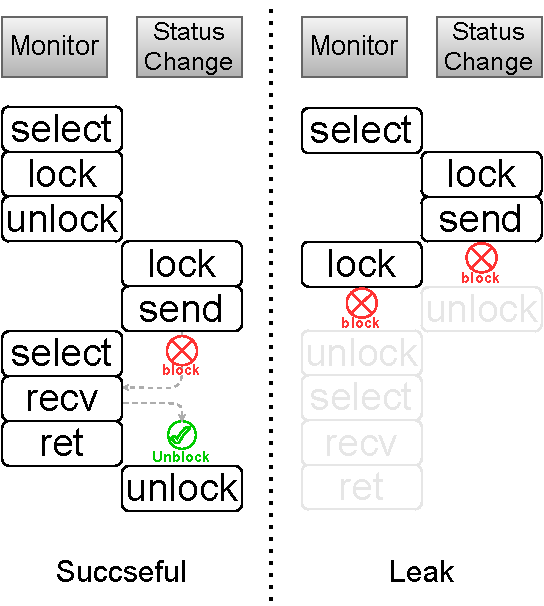
\includegraphics[width=.99\linewidth]{goat/figs/execViz_moby.pdf}
\end{minipage}
\caption{Simplified version of bug \texttt{moby28462}}
\label{listing:moby28462.minipage}
\end{listing}

%\begin{listing}[]
\begin{minipage}{.45\columnwidth}
\begin{minted}
[
fontsize=\footnotesize,
linenos=true,
escapeinside=||,
xleftmargin=2em,
breaklines
]
{go}
package main
import "sync"

type Cont struct{|\label{bugListing:containerType_start}|
  sync.Mutex
  stop  chan struct{}
}|\label{bugListing:containerType_end}|

func main() {
  cnt := &Cont{|\label{bugListing:container_create_start}|
       stop:make(chan struct{})}|\label{bugListing:container_create_end}|
  go Monitor(cnt)|\label{bugListing:main_go_monitor}|
  go StatusChange(cnt)|\label{bugListing:main_go_statChange}|
}
\end{minted}
\end{minipage}\hfill
\begin{minipage}{.45\columnwidth}
\begin{minted}
[
fontsize=\footnotesize,
linenos=true,
escapeinside=||,
breaklines
]
{go}
|\setcounter{FancyVerbLine}{15}|func Monitor(cnt *Cont){
  for{
    select{
    case <- cnt.stop:  |\label{bugListing:Monitor_case_recv}|
      return |\label{bugListing:Monitor_case_recv_ret}|
    default: |\label{bugListing:Monitor_case_def}|
      cnt.Lock()  |\label{bugListing:Monitor_case_def_lock}|
      cnt.Unlock() |\label{bugListing:Monitor_case_def_unlock}|
}}}
func StatusChange(cnt *Cont){
  cnt.Lock() |\label{bugListing:statChange_lock}|
  defer cnt.Unlock() |\label{bugListing:statChange_defer_unlock}|
  cnt.stop <- struct{}{} |\label{bugListing:statChange_send}|
}
\end{minted}
\end{minipage}
\caption{Simplified version of bug \texttt{moby28462}}
\label{listing:moby28462.minipage.codeOnly}
\end{listing}


\subsection{Go Concurrency}
\label{sec:goConcurrency}
%
Go introduces a new concurrency model, mixing shared-memory features of languages like Java/C/C++ and message-passing concepts such as Erlang's, with an ad-hoc scheduler that orchestrates Go's concurrent components interactions while shielding the user from many low-level aspects of the runtime.
%
The language is equipped with a rich vocabulary of \textit{serialization} features to facilitate the memory model constraints~\cite{go-memModel}; they include synchronous and asynchronous communication, memory protection, and barriers for efficient synchronization:
\begin{itemize}
    \item \textbf{Goroutines} are functions that execute concurrently on logical processors having their own stack.
    \item \textbf{Channels} are typed conduits through which goroutines communicate.  Channels are unbuffered by default, providing synchronous (rendezvous) or asynchronous (via buffered channels) messaging between goroutines.
    \item \textbf{Synchronization} features such as \textit{(RW)mutex}, \textit{waitGroup}, \textit{conditional variables}, \textit{select}, and \textit{context} are included in the language to provide more and flexible synchronization, data access serialization, memory protection, and error handling.
    \item \textbf{Scheduler} maintains goroutines in FIFO queues and binds them on OS threads to execute on processing cores.
\end{itemize}


This design facilitates the construction of data flow models that efficiently utilize multiple CPU cores and encourages developers to \textit{share memory through communication} for safe and straightforward concurrency and parallelism.
%
This rich mixture of features has, unfortunately, greatly exacerbated the complexity of debugging.
%
In fact, the popularity of Go has outpaced its debugging support~\cite{go-survey,tu-concurrentBugs-asplos19,yuan-gobench-cgo21}.
%
There are some encouraging developments in support of debugging, such as a data race checker \cite{go-race-blog} that has now become a standard feature of Go and has helped catch many a bug.
%
However, the support for blocking bugs such as deadlocks and Go-specific bug-hunting support for Go idioms (e.g., misuse of channels and locks) remain insufficiently addressed.



%\begin{listing}[]
\centering
\begin{minted}
[
fontsize=\scriptsize,
linenos=true,
escapeinside=||,
breaklines
]
{go}
package main
import "sync"

type Container struct{ |\label{bugListing:containerType_start}|
  sync.Mutex
  stop  chan struct{}
} |\label{bugListing:containerType_end}|

func main() {
  container := &Container{ |\label{bugListing:container_create_start}|
       stop:make(chan struct{})} |\label{bugListing:container_create_end}|
  go Monitor(container) |\label{bugListing:main_go_monitor}|
  go StatusChange(container) |\label{bugListing:main_go_statChange}|
}
%|\setcounter{FancyVerbLine}{15}|func Monitor(cnt *Container){
func Monitor(cnt *Container){
  for{
    select{
    case <- cnt.stop:  |\label{bugListing:Monitor_case_recv}|
      return |\label{bugListing:Monitor_case_recv_ret}|
    default: |\label{bugListing:Monitor_case_def}|
      cnt.Lock()  |\label{bugListing:Monitor_case_def_lock}|
      cnt.Unlock() |\label{bugListing:Monitor_case_def_unlock}|
}}}
func StatusChange(cnt *Container){
  cnt.Lock() |\label{bugListing:statChange_lock}|
  cnt.stop <- struct{}{} |\label{bugListing:statChange_send}|
  cnt.Unlock() |\label{bugListing:statChange_defer_unlock}|
}
\end{minted}
\caption{Simplified version of bug \texttt{moby28462}}
\label{listing:moby28462}
\end{listing}


%\stcmtside{Explaining the example to motivate}
Listing \ref{listing:moby28462.minipage} shows a simplified version of a reported bug in Docker \cite{moby-28462-commit}.
%
An instance of the \texttt{Container} type (lines \ref{bugListing:containerType_start}-\ref{bugListing:containerType_end}) is created in the \texttt{main} function (lines \ref{bugListing:container_create_start}-\ref{bugListing:container_create_end}).
%
In line \ref{bugListing:main_go_monitor}, a goroutine is spawned to execute function \texttt{Monitor} that continuously checks the container status and returns once it receives from the container's channel (lines \ref{bugListing:Monitor_case_recv}-\ref{bugListing:Monitor_case_recv_ret}).
%
The default case of the \texttt{select} statement (line \ref{bugListing:Monitor_case_def}) allows \texttt{Monitor} to continue monitoring without getting blocked on the channel receive (line \ref{bugListing:Monitor_case_recv}).
%
Concurrent to the \texttt{main} and \texttt{Monitor} goroutines, another goroutine is created in line  \ref{bugListing:main_go_statChange} to execute function \texttt{StatusChange} which changes the status of the container by sending to the container's channel.
%
The container's lock is released after the send action completes and function returns (\texttt{defer} statement in line \ref{bugListing:statChange_defer_unlock}).
%


Native execution of this program terminates successfully without issuing any error or warning.
%
Based on the Go specification and memory model, there is no constraint on the goroutines spawned from the \texttt{main} function to join back before the \texttt{main} goroutine\footnote{In the remainder of the paper, we use \textit{main function} and \textit{main goroutine} interchangeably.} terminates.
%
A deadlock detector within the runtime periodically checks that the scheduler queues of all \textit{runnable} goroutines never become empty until the \texttt{main} goroutine terminates.
%
In other words, the runtime throws a deadlock exception when the \texttt{main} goroutine is blocked, and no other goroutine is in the queue to execute (\ie \textit{global deadlock}).
%
Since there is no blocking instruction in the \texttt{main} goroutine in listing \ref{listing:moby28462.minipage}, the program terminates successfully regardless of other goroutines' statuses.
%
However, this program suffers from a common bug in concurrent Go where one or more goroutines \textit{leak} (\ie, \textit{partial deadlock}) from the execution (\ie, never reach their end states).

%\stcmtside{Explain the deadlock (leak) situation that might get overlooked}
%Due to the non-determinism introduced by the runtime scheduler and application-level random features like \texttt{select}, many interleavings are feasible for concurrent execution of simple programs such as listing \ref{listing:moby28462.minipage}.
%
The right side of the listing displays a successful run and a leak situation of the program.
%
In the leak situation, first, the \texttt{Monitor} goroutine executes the \texttt{select} statement and, based on the available cases, picks the default case to execute.
%
Right before the execution of mutex lock (line \ref{bugListing:Monitor_case_def_lock}), the scheduler context-switches and the \texttt{StatusChange} goroutine starts its execution through which it holds the lock and blocks on sending to the channel (line \ref{bugListing:statChange_send}) since there is no receiver on that channel.
%
Upon blocking on send, the scheduler transfers back the control to the \texttt{Monitor} goroutine that tends to acquire the mutex, but because the mutex is already held by \texttt{StatusChange}, the \texttt{Monitor} goroutine also blocks.
%
The circular wait between the container mutex and channel prevents both spawned goroutines from reaching their end states and leaves the program in an unnoticed deadlock situation.
%
%\stcmtside{The thirst for novel and scalable debuggers}
%Widely used deadlock detectors such as Goodlock \cite{havelund-goodlock-spin00} are not applicable in Go since causes of Go deadlocks are resources (\eg, locking a locked mutex) or communication (\eg, sending on a full channel), or a combination of them (\eg, leaky interleaving of listing \ref{listing:moby28462.minipage}).
%
%In addition, due to the lightweight nature of goroutines, it is not uncommon to spawn thousands of goroutines in production software systems.
%
%Hence,  novel and scalable techniques are needed to enable realistic modeling of program behavior during execution.
%

\subsection{Concurrency Bugs in Go}
\label{sec:goBugs}
Based on a proposed bug taxonomy for Go \cite{tu-concurrentBugs-asplos19}, bugs are categorized separately based on their \textit{causes} (shared-memory vs. message-passing) and \textit{symptoms} (blocking vs. non-blocking).
%
Blocking bugs historically refer to situations where one or more processing units (\eg, goroutines) are blocked, waiting for an external signal to resume (\eg, leak situation in listing \ref{listing:moby28462.minipage}.
%
The observed causes of such blocking flaws in the context of Go are as follows:

\begin{itemize}
  \item \textit{Resource deadlocks}: Go inherits resource deadlocks from multithreaded languages like Java and C/Pthreads where goroutines are trapped in a circular wait for the resource (\eg, mutex) that is held by other goroutines.
  \item \textit{Communication deadlocks}: Synchronized (unbuffered) channels transmit values from one goroutine to another in a rendezvous fashion. The sender (or receiver) blocks until the receiver (or sender) is ready to receive (send). Misuse of channel operations might result in one or more goroutines waiting for a sender/receiver to unblock them forever.
  \item \textit{Mixed deadlocks}: The leak situation in listing \ref{listing:moby28462.minipage} is the example of such deadlocks where one goroutine is blocked on acquiring a resource that is held by another goroutine which is blocked on communication.
\end{itemize}

Similar to other concurrent languages, Go has non-blocking bugs such as data races and atomicity violations while introducing new bug idioms due to its new concepts such as anonymous functions \cite{tu-concurrentBugs-asplos19}.
%
This work focuses on blocking bugs (i.e., partial and global deadlocks).

%\stcmt{below: Application-level non-determinism makes debugging more difficult}
%\noindent{\bf Application-level non-determinism:\/}
In addition to the non-deterministic nature of concurrent languages caused by the scheduler and interaction between concurrent components, Go introduces some level of non-determinism at the application level.
%
The \textit{select-case} statement (similar to switch-case) allows the goroutine to wait on multiple channel operations.
%
The runtime picks one case pseudo-randomly among available cases (\ie, channel sends and receives that are ready to execute without blocking).
%
If none of the cases are ready, the executing goroutine is blocked unless there is a \textit{default} case.
%
The default case makes the select non-blocking and prevents the goroutine from waiting for unavailable communications.
%
Such random behavior expands the interleaving space, and it grows exponentially when nested selects are employed in conjunction with nested loops.
%
As a result, tracing the cause of a program's misbehaved execution becomes increasingly tricky.
%
Our observations (section \ref{sec:ch4_evaluation}) demonstrate that \textbf{select statements are involved at the center of many rare bugs}.


\subsection{Accelerating Bug Exposure}
Blocking bugs are primarily caused by the non-deterministic decisions that the scheduler makes.
%
Such bugs may not manifest themselves in conventional testing and are difficult to reproduce.
%
Figure \ref{fig:rare_bugs} displays the histogram of 68 blocking bug kernels grouped by the number of trials that \goat takes to detect them.
%
Approximately 30\% of bugs required more than one execution to happen and be detected by \goat\footnote{The figure and numbers are obtained from trials of \goat on native execution of bug kernels without any randomization (\ie, $D=0$).}.
%
\textit{stress testing} is a common way to detect such rare bugs by exercising the scheduler and examine the program's behavior in many executions.
%
However, such testing is inefficient because some interleavings might get tested repeatedly while other feasible interleavings remain untested.
%
It has been empirically demonstrated that a small amount of randomness in each test execution can drastically reduce the number of iterations needed to find concurrency bugs \cite{thomson-concurrencyTesting-ppopp14,emmi-delayBounded-popl11}.
%
For instance, forcing context-switches before synchronization/serialization operations in concurrent programs increases the probability of finding rare concurrent bugs \cite{burckhardt-depthBug-asplos10}.
%
In listing \ref{listing:moby28462.minipage}, a rare context-switch after the \texttt{select} statement in line \ref{bugListing:Monitor_select} causes the lock operation on mutex $m$ in line \ref{bugListing:Monitor_case_def_lock} of goroutine \texttt{Monitor} to \textit{block} goroutine \texttt{StatusChange} on locking $m$ in line \ref{bugListing:statChange_lock} and causing a deadlock.
%
Concurrency primitive usages (\eg, channel send/recv, mutex lock/unlock, select) are the \textit{critical points} in the program because their behavior directly impacts the blocking behavior of Go programs.
%
In \goat, we statically identify such critical points and inject \textit{yield} handlers before each concurrency primitive usage.
%
During execution, the handlers randomly decide if the current goroutine should yield to other goroutines to execute.
%
Results in section \ref{sec:ch4_evaluation} show that such simple yields are effective in detecting rare bugs.

\subsection{Testing Coverage Analysis}
\label{sec:coverage}
To demonstrate that testing has been thorough, \textit{coverage metrics} are defined to measure the progress of tests and specify testing termination conditions.
%
Coverage metric for the set of testing executions $\mathcal{T}$ is a set of \textit{requirements} $\mathcal{R}$ that should get covered during testing iterations.
%
We say requirement $R_i \in \mathcal{R}$ is covered during testing iteration $t_j \in \mathcal{T}$ if we can correlate an \textit{action} during execution of $t_j$ to $R_i$.
%
For example, in \textit{statement coverage}, which is a widely-used metric in testing sequential software, $R$ is the set of source locations (file and line numbers) in the target program.
%
$R_i$ is covered by test execution $t$ if the statement at location $R_i$ is executed in $t$.
%
The \textit{coverage percentage} of a test $\mathcal{T}$ is the ratio of the requirements covered by at least one execution over the number of all requirements ($|R|$).

Concurrent software testing frameworks perform testing iterations to explore the schedule space and expose flaws.
%
Depending on the class of target bug, different coverage metrics are proposed to quantify the quality of search space exploration.
%
\textit{Synchronization} coverage metrics such as \textit{blocking-blocked} \cite{edelstein2003contest}, \textit{blocked-pair-follows} \cite{trainin-followsCoverage-padtad09} and \textit{synchronization-pair} \cite{hong-syncTesting-issta12} defined requirements to cover during testing for exposing blocking bugs (\eg deadlocks).
%
%\textit{Memory access} coverage metrics such as PSet \cite{yu-pser-isca09} and def-use \cite{yang-defuse-issta98} focuses on data-access related bugs such as atomicity violation or data races.
%
For example, the synchronization coverage model in \cite{edelstein2003contest} defines \textit{blocking} and \textit{blocked} requirements per each synchronized block (\ie mutually exclusive section of the code that is protected by a lock).
%
The purpose of this requirement is to check if a test can report when there is a lock contention for two or more threads entering the synchronized block.
%
That is, a thread is either \textit{blocked} from entering the synchronization block or \textit{blocking} other threads from entering by holding the lock.
%



\begin{figure}[t]
\begin{minipage}{.49\textwidth}
\centering
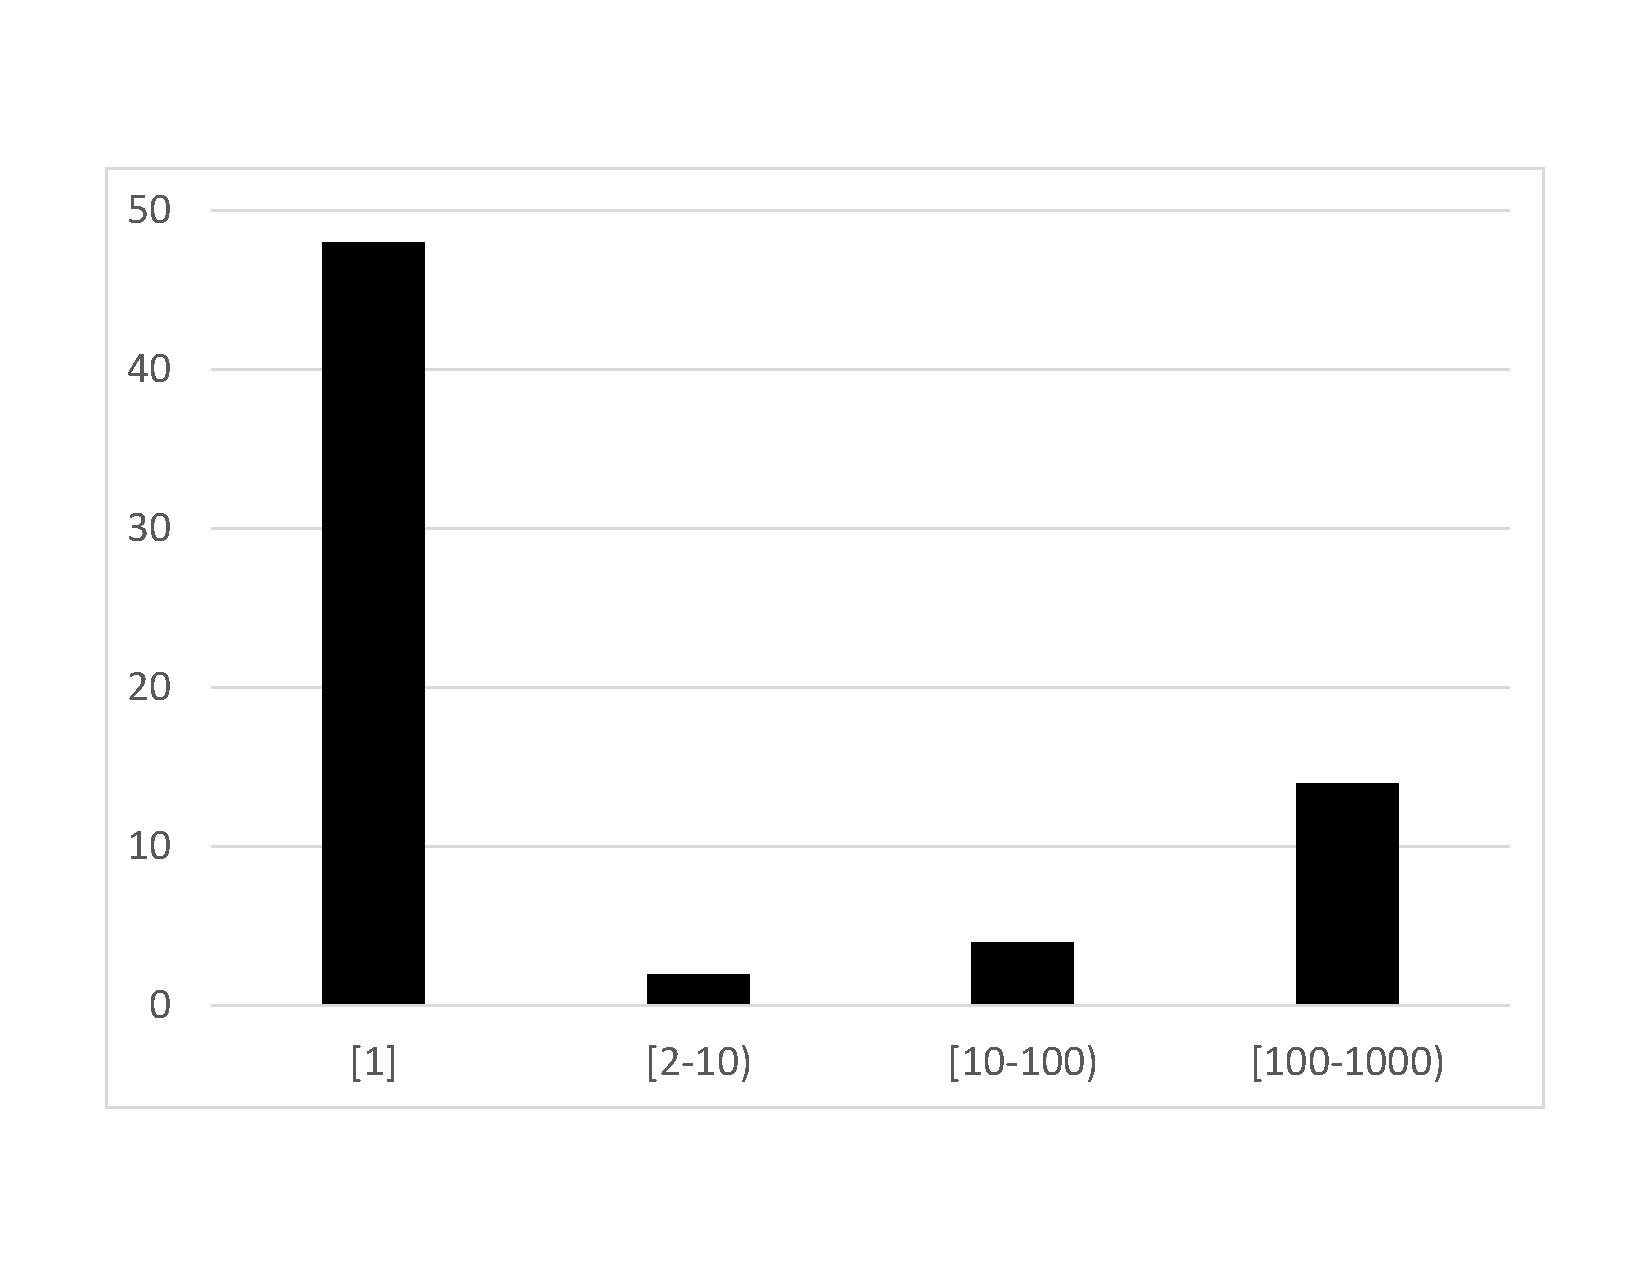
\includegraphics[width=0.9\linewidth]{goat/figs/coverage_motivation.pdf}
%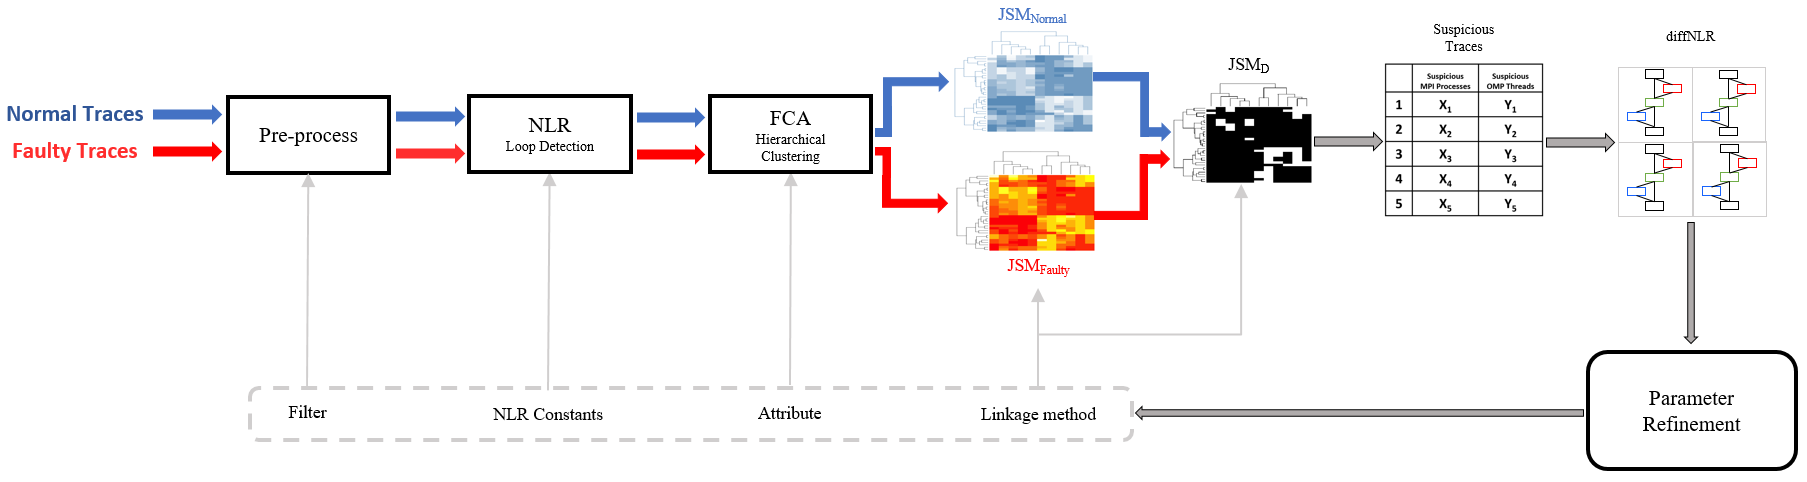
\includegraphics[]{figs/overview.png}
%\includegraphics[]{figs/overv}
\caption{Distribution of number of trials for \goat (D0) to detect 68 blocking bugs in GoKer~\cite{yuan-gobench-cgo21}}
\label{fig:rare_bugs}
\end{minipage}
\begin{minipage}{.49\textwidth}
\centering
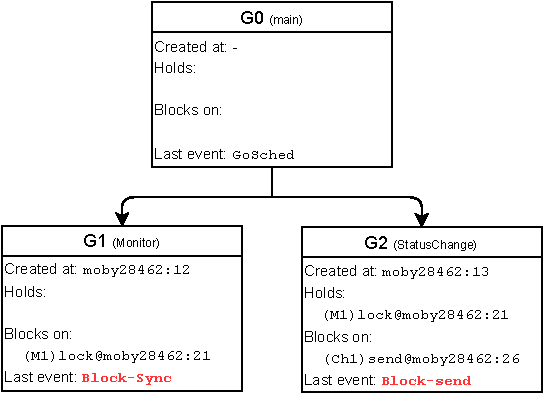
\includegraphics[width=0.9\linewidth]{goat/figs/gtree.pdf}
%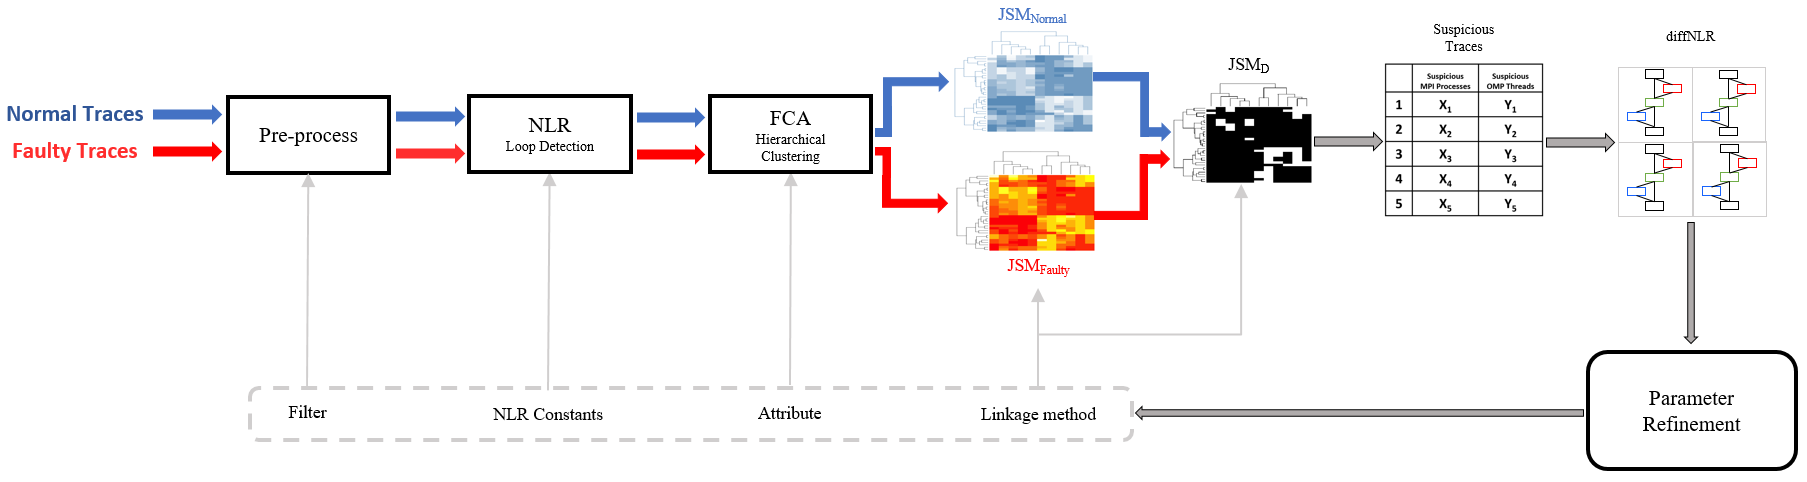
\includegraphics[]{figs/overview.png}
%\includegraphics[]{figs/overv}
\caption{Goroutine tree of the leak situation in listing \ref{listing:moby28462.minipage}}
\label{fig:gtree}
\end{minipage}
\end{figure}


The existing concurrency coverage metrics are primarily in the context of Java and C/Pthreads.
%
They are not necessarily applicable to languages like Go as such languages have different concurrency primitives and semantics.
%
Novel coverage metrics are required to enable the quantification of interleaving space exploration.
%
Bron et al.,\cite{bron-appSyncCov-ppopp05} enumerates four major characteristics for coverage metrics to gain acceptance:
\begin{enumerate}
  \item \textbf{Static model:} A static model of requirements from the given program should be constructed by instrumenting the source code. The model should be well-understood by the developer or tester before execution. The model should maintain covered requirements during testing executions.
  \item \textbf{Coverable and measurable requirements:} The absolute majority of requirements should be realistic enough to be \textit{coverable} during testing. For a few that are not coverable (due to program semantics) or not \textit{measurable} (because of technical limitations), the developer should be aware of the reason.
  \item \textbf{Actions for uncovered requirements:} After testing terminates, every uncovered requirement should yield an action (\eg, extending testing iterations or removing dead code from the program, thus removing uncoverable requirements)
  \item \textbf{Coverage satisfaction:} Some action should be taken upon reaching a threshold of coverage percentage (e.g., testing phase termination when reaching 100\% statement coverage)
\end{enumerate}

Defining a new coverage metric to satisfy the above characteristics requires an accurate and proper mental model of target bugs.
%
Using the \goat's infrastructure, we studied the underlying causes of many bugs, including GoKer benchmark~\cite{yuan-gobench-cgo21} and propose a set of coverage requirements that enables extensive analysis of dynamic behavior of concurrency primitives under various scheduling scenarios.
%
In section \ref{sec:ch4_covreq}, we describe our proposed coverage metric for testing concurrent Go, which are extensible to all concurrent languages.


\section{Design and Implementation}
\label{sec:ch4_design}
\subsection{Overview}
\label{sec:ch4_overview}
Figure \ref{fig:goat_workflow} displays the overview of \goat.
%
Given a program \textbf{P} (\ie, a set of Go source files with a \textit{main} function), \goat automatically instruments \textbf{P} and constructs static and dynamic models of execution for thorough testing and analysis.
%
Our main goal in \goat is to facilitate the investigation of \textit{non-deterministic interactions between concurrent components} (\ie, concurrent behavior) of \textbf{P} to achieve objectives acquainted in section \ref{sec:ch4_intro}.
%
\\
\noindent{\bf Static Analysis:\/} (section \ref{sec:ch4_static_analysis})---
\goat statically constructs a model \textbf{M} which is a table of source locations (files and line numbers) associated with concurrency primitive usages in \textbf{P} source files.
%
The primary use of \textbf{M} is to identify locations in \textbf{P} as potential points for manipulating the schedule to explore possible scenarios and accelerate the discovery of rare bugs.
%
Yield handlers are injected before each entry in \textbf{M} to decide if the following concurrency action (\eg, message send or mutex lock) should perform or yield to other goroutines.
%
Such yields effectively perturb the scheduler and execute feasible but unconventional interleavings of \textbf{P}.
%
\\
\noindent{\bf Coverage Requirements:\/} (section \ref{sec:ch4_covreq})---
Forcing the schedule perturbation is effective for exploring the feasible interleaving space until the bug is hit.
%
However, a metric is required to evaluate the quality of interleaving space exploration and measure the progress until reaching a threshold.
%
Following the factors of effective coverage metrics, we employ \textbf{M} to emulate the possible behavior of concurrent components of \textbf{P} and define a set of \textit{coverage requirements} as indicators for quality and progress of schedule space exploration.
%
The requirements are defined so that, during testing, a lack of requirement demands the user to fix the bug or remove the dead code.
\\
\noindent{\bf Dynamic Analysis:\/} (section \ref{sec:ch4_dynamic_tracing})---
To gain insight into the concurrent behavior of \textbf{P} and measure the covered requirements, we equipped \goat with a dynamic tracing mechanism, which is an extension to the Go standard tracer package~\cite{go-cmd-trace}.
%
When tracing is enabled, an \textit{execution concurrency trace} (ECT) file is generated once the execution of \textbf{P} terminates (\eg, successfully exits, fails, times out).
%
ECT is a totally ordered \textit{sequence} of events that contain information about the dynamic behavior concurrent components, enabling offline analysis of \textbf{P}'s execution.
\\
\noindent{\bf Offline Analysis:\/} (section \ref{sec:ch4_offline_analysis})---
In offline, \goat first, separates the application-level events of ECT from the underlying runtime system of Go.
%
Then, it constructs a goroutine tree from application-level goroutines to check if any goroutine has leaked/blocked (\ie, did not reach its final state) after the execution termination.
%
Additionally, \goat maintains a global goroutine tree for \textbf{P} and equivalences goroutines from run to run to accumulate the covered requirements from each execution of \textbf{P}.
%
As soon as a bug is detected or the coverage exceeds a threshold, \goat stops running and produces reports for manual analysis by the user.
%

\subsection{Static Analysis}
\label{sec:ch4_static_analysis}

\subsubsection{Concurrency Usage Model}
\goat statically constructs a model \textbf{M} from the usage of concurrency primitives in \textbf{P} files which enables uniform analysis during testing iterations.
%
\textbf{M} is a table of source locations (files and line numbers) associated with \textit{concurrency usages} (CU).
%
We define CU as a triple of $(f,l,k)$ where $f$ is the file name, $l$ is the line number, and $k$ is the concurrency primitive used in the code location.
$k\in$ \texttt{Channel} $\cup$ \texttt{Sync} $\cup$ \texttt{Go} where:
\begin{itemize}
  \item \texttt{Channel} = \{\texttt{send}, \texttt{receive}, \texttt{close}\}
  \item \texttt{Sync} = \{\texttt{lock}, \texttt{unlock}, \texttt{wait}, \texttt{add}, \texttt{done}, \texttt{signal}, \texttt{broadcast}\}
  \item \texttt{Go} = \{\texttt{go}, \texttt{select}, \texttt{range}\}
\end{itemize}

\goat constructs \textbf{M} by traversing the \textit{abstract syntax tree} (AST) for each file in \textbf{P} using the Go AST package~\cite{go-package-ast}.
%
The first column of table \ref{tab:moby_cov_table} shows the CU locations extracted from program in listing \ref{listing:moby28462.minipage}.

\subsubsection{Source Instrumentation}

We employ \textbf{M} entries to instrument \textbf{P} with tracing and schedule perturbation mechanisms.
%
First, we traverse the AST of \textbf{P} and inject three statements (\ie, AST nodes) to the beginning of \textbf{P}'s main function to enable end-to-end tracing:
\begin{itemize}
  \item \texttt{goat\_done := goat.Start()} initializes \goat, enables tracing, and returns a channel as a conduit between application space and \goat.
  \item \texttt{go goat.Watch(goat\_done)} spawns a new goroutine as a watchdog for the liveness of the program (in case of global deadlock or infinite loop). The watchdog goroutine either receives from \texttt{goat\_done} and sends back an ack signal or timeouts (default: 30 seconds). Then it stops tracing, flushing the trace buffer, and terminates.
  \item \texttt{defer goat.Stop(goat\_done)} sends a value to the watcher goroutine after main returns and signals that the program is finished. Then it waits to receive the signal from the watcher, then stops tracing and terminates.
\end{itemize}

Moreover, we inject calls to \texttt{goat.handler()} before each CU in \textbf{M} to manipulate the native scheduler around concurrency primitve usages. \texttt{goat.handler()} is a function invocation that randomly calls \texttt{runtime.GoSched()} within a bound $D$ to preempt the processing core from current goroutine and push the goroutine to the back of the global queue of runnable goroutines.
%
When $D=0$, \goat does not perturb the scheduler and lets \textbf{P} to execute natively. For any $D>0$, \goat manipulates application-level goroutines from their regular execution D times.
%
Our experiments (section \ref{sec:ch4_evaluation}) demonstrate that the optimum value for $D$ is not larger than 3, showing that even a small number of yields is effective in exposing the bug (as also shown in \cite{burckhardt-depthBug-asplos10}).

\subsection{Coverage Requirements}
\label{sec:ch4_covreq}
Based on our investigations from the execution of Go applications and bug kernels, we emulate the possible behavior of concurrent components by defining a set of coverage requirements (summarized in table \ref{tab:cov_req}):
%
\begin{itemize}
  \item \textbf{Req1 (Send/Recv):} \{\texttt{blocked}, \texttt{unblocking}, \texttt{NOP}\} -- Goroutine $G_1$ is either \textit{blocked} on a channel send (receive) if the receiver (sender) goroutine $G_2$ is not ready, or \textit{unblocking} the waiting receiver (sender) goroutine $G_2$. A channel send or receive might also be neither blocked nor unblocking (NOP) for buffered channels.
  \item \textbf{Req2 (Select-Case):} \{\texttt{blocked}, \texttt{unblocking}, \texttt{NOP}\} $\times$ \{\texttt{case}$_i$\} -- cases of select statements are channel sends and recives (or default case for non-blocking selects). For all select statements that has no default case, we obtain the cases of each select statement at runtime and maintain an instance of Req1 per case.
  \item \textbf{Req3 (Lock):} \{\texttt{blocked}, \texttt{blocking}\} -- Goroutine $G_i$ is either \textit{blocked} when locking a mutex because another goroutine has locked the mutex or \textit{blocking} other goroutines from acquiring the mutex lock.
  \item \textbf{Req4 (Unblocking):} \{\texttt{unblocking}, \texttt{NOP}\} -- The goroutine that is performing channel close, mutex unlock, conditional variable signal and broadcast, waitGroup done, and non-blocking select case (send or receive) either \textit{unblocks} one or more blocked goroutines or has no effect (NOP).
  \item \textbf{Req5-Go:} \{\texttt{NOP}\} -- We emit a NOP action for each goroutine creation to indicate that it is covered during testing.
\end{itemize}


\begin{table}[b]
\centering
\caption{Coverge requirements defined for concurrent Go}
\scalebox{0.83}{
\begin{tabular}{|
>{\columncolor[HTML]{FFFFFF}}l |
>{\columncolor[HTML]{FFFFFF}}l |
>{\columncolor[HTML]{FFFFFF}}c |
>{\columncolor[HTML]{FFFFFF}}c |
>{\columncolor[HTML]{FFFFFF}}c |
>{\columncolor[HTML]{FFFFFF}}c |}
\hline
\multicolumn{1}{|c|}{\cellcolor[HTML]{FFFFFF}} & \multicolumn{1}{c|}{\cellcolor[HTML]{FFFFFF}} & \multicolumn{4}{c|}{\cellcolor[HTML]{FFFFFF}Coverage Requirement Types} \\ \cline{3-6}
\multicolumn{1}{|c|}{\multirow{-2}{*}{\cellcolor[HTML]{FFFFFF}\begin{tabular}[c]{@{}c@{}}Coverage\\ Requirements\end{tabular}}} & \multicolumn{1}{c|}{\multirow{-2}{*}{\cellcolor[HTML]{FFFFFF}\begin{tabular}[c]{@{}c@{}}Concurrent\\ Action\end{tabular}}} & Blocked & Unblocking & Blocking & NOP \\ \hline
\cellcolor[HTML]{FFFFFF} & SEND & * & * &  & * \\ \cline{2-6}
\multirow{-2}{*}{\cellcolor[HTML]{FFFFFF}Req. 1: Send/Recv} & RECV & * & * &  & * \\ \hline
\cellcolor[HTML]{FFFFFF} & CASE$_i$ (SEND) & * & * &  & * \\ \cline{2-6}
\multirow{-2}{*}{\cellcolor[HTML]{FFFFFF}Req. 2: Select-Case} & CASE$_i$ (RECV) & * & * &  & * \\ \hline
Req. 3: Lock & LOCK & * &  & * &  \\ \hline
\cellcolor[HTML]{FFFFFF} & CLOSE &  & * &  & * \\ \cline{2-6}
\cellcolor[HTML]{FFFFFF} & UNLOCK &  & * &  & * \\ \cline{2-6}
\cellcolor[HTML]{FFFFFF} & SIGNAL &  & * &  & * \\ \cline{2-6}
\cellcolor[HTML]{FFFFFF} & BRDCST &  & * &  & * \\ \cline{2-6}
\multirow{-5}{*}{\cellcolor[HTML]{FFFFFF}Req. 4: Unblocking} & NB-SELECT &  & * &  & * \\ \hline
Req. 5: Go & Go &  &  &  & * \\ \hline
\end{tabular}

}
\label{tab:cov_req}
\end{table}

%
With the help of \goat's infrastructure, the proposed requirements satisfy the characteristics of an ``acceptable'' coverage metric because:
\begin{enumerate}
  \item A \textit{static model} \textbf{M} from program \textbf{P} is obtained by identifying its CU points. \textbf{M} is easy to understand by developers and reflects the concurrent behavior of \textbf{P}.
  \item The defined requirements are \textit{measurable} by analyzing the test's ECT. A global data structure maintains the covered requirements by each $t \in \mathcal{T}$.
  \item Upon completion of $\mathcal{T}$ iterations, the \textit{uncovered} requirements imply some \textit{meaningful} information about the behavior of \textbf{P}. For example, if a send is always performing as \textit{unblocking} and never as \textit{blocked}, it means that the receiver always performs receive before the sender reaches its send instruction. In other words, the receive action \textit{always happen-before} send action. This communication pattern might be part of \textbf{P}'s semantics and matches the developer's expectations (e.g., a set of goroutines are listening on a channel to perform non-frequent requests). Otherwise, the uncovered requirement  ``send-\texttt{blocked}'' reflects a bug or flaw in the program design.
  \item Since \goat can detect occurred blocking bugs and maintain a global coverage model, $\mathcal{T}$ iterations terminate either by detecting a bug or reaching a coverage percentage threshold.
\end{enumerate}

\subsection{Dynamic Concurrency Tracing}
\label{sec:ch4_dynamic_tracing}
The standard execution tracer package \cite{go-package-trace,go-cmd-trace} provides dynamic tracing for the construction of execution models from the interactions of processors, OS threads, goroutines, the scheduler, and the garbage collection mechanism.
%
The tracing mechanism is compiled into all programs always through the runtime and is enabled on demand to study \textit{perfromance bottlenecks} through visualizers like \textit{pprof} \cite{go-profile-blog}.
%
The alphabet of trace events is total of 49 events \cite{goParserSource}, categorized and summarized in table \ref{tab:events}.
%
Although the event vocabulary is rich enough to model comprehensive goroutine latency and blocking behavior accurately,
the vocabulary lacks concurrency primitive usage events for the construction of concurrency models.
%
We enrich the standard tracing mechanism with 14 additional events to enable the production of dynamic models from the program's concurrency behavior:
\begin{itemize}
    \item \textbf{Channel:} For each channel operation (make, send, receive, close), ECT includes an event with a unique id assigned to each channel.
    \item \textbf{(RW)Mutex, WaitGroup \& Conditional Variables:} Similar to channels, we assign a unique id to each concurrency object and emit an event for each of their operations (lock, unlock, rlock, runlock, add, wait, signal, broadcast).
    \item \textbf{Select \& Schedule:} The scheduler and the \textit{select} structure introduce non-determinism to the execution. We keep track of the decisions made by the scheduler and select statements to obtain an accurate decision path during execution.
\end{itemize}

We call the output of enhanced tracer \textit{execution concurrency trace} (ECT).
%
ECT is a totally ordered \textit{sequence} of events in which the order is approximated through a central clock with nanosecond precision.
%
ECT also contains the call-stack for each event, enabling a direct mapping of events to source-line numbers.
%
For each blocking operation (channels \textit{sends}/\textit{recvs}, mutex \textit{locks}, waitGroup/conditional variable \textit{wait} and \textit{select} (when none of the cases are available)), ECT captures a pair of pre-operation and post-operation events to distinguish between the \textit{request for action} and \textit{completion of action}.
%
Hence, ECT is especially effective for debugging because it enables modeling the blocking state of concurrent components at any given step of program execution.
%
The enhanced dynamic tracing also enables the measurement of coverage requirements in offline (section \ref{sec:ch4_offline_analysis}).

\begin{table}[t]
    \centering
        \caption{Event categories by the Go execution tracer}
        \begin{tabular}{|l|l|}
        \hline
        \rowcolor[HTML]{C0C0C0}
        \multicolumn{1}{|c|}{\cellcolor[HTML]{C0C0C0}\textbf{Category}} & \multicolumn{1}{c|}{\cellcolor[HTML]{C0C0C0}\textbf{Description}} \\ \hline
        Process & Indication of process/thread start and stop \\ \hline
        GC/Mem & Garbage collection and memory operation events\\ \hline
        Goroutine & Goroutines events: create, block, start, stop, end, etc. \\ \hline
        Syscall & Interactions with system calls \\ \hline
        Users & User annotated regions and tasks (for bounded tracing) \\ \hline
        Misc & System related events like futile wakeup or timers \\ \hline
        \end{tabular}
    \label{tab:events}
\end{table}



\subsection{Offline Analysis}
\label{sec:ch4_offline_analysis}
In the lifetime of Go programs' executions, the runtime system creates new goroutines or pick from the pool of dead goroutines to perform various tasks such as bootstrapping the program, garbage marking and sweeping, and tracing.
%
\goat also adds an extra goroutine to \textit{watch} the program execution in case of the main goroutine blockage.
%
These goroutines are captured during tracing, but our focus is on the goroutines created from within the application.
%
The distinguishment between runtime goroutines and application goroutines is essential to define the boundaries of the application and separate them from the underlying system.
%
We say a goroutine is an \textit{application-level} goroutine if it is the main goroutine (that executes the main function) or it has all of the following conditions:
1) its ancestor is the main goroutine,
2) it is not a Go runtime system goroutine, and
3) it is not a tracer goroutine.
These conditions are assessed for every captured goroutine in ECT by checking the call stack of their corresponding $GoCreate$ event.

\goat constructs a \textit{goroutine tree} (figure \ref{fig:gtree}) of application-level goroutines from the generated ECT.
%
Nodes in the goroutine tree represent a goroutine, and directed edges denote parent-child relationships in which the child is created from a \texttt{go} statement that the parent executes.
%
Each node of the tree contains the entire sequence of events that the goroutine executed \footnote{The sequence of events per node is not shown in figure \ref{fig:gtree} for simplicity.}, information about the goroutine's creation site, the resources it holds at each execution point, and the final executed event right before the program termination.
%
\goat analyzes this collection of information to check whether any goroutine leaked after termination and whether the coverage requirements are covered.

\subsubsection{Leak Detection}
When tracing is enabled, every application goroutine invokes the tracer to capture $GoEnd$ before finishing its execution.
%
Before the main function returns, the main goroutine hands over the control to the root goroutine to finalize the program termination.
%
This context-switch is done through invocation of \texttt{runtime.Gosched()} which emits the $GoSched$ event.
%
In \goat, the main goroutine's final event in a successful execution is $GoSched$ with \texttt{runtime.traceStop} on top of its stack.

We call an execution \textbf{successful}, if below conditions hold:
\begin{enumerate}
  \item (1) all goroutines spawned in the main goroutine has $GoEnd$ as their final event
  \item (2) the final event of the main goroutine is $GoSched$ with \texttt{runtime.traceStop} on top of its stack.
\end{enumerate}

In the absence of any of these conditions, we conclude that the program suffers from a ``deadlock'' bug, because at least one goroutine did not reach its final state.
%
Therefore, \goat executes procedure \ref{proc:deadlockCheck} which is a BFS traversal on the goroutine tree to check if the program suffers from partial or global deadlocks.


\begin{small}
\begin{algorithm}[b]
 \DontPrintSemicolon
 \SetKwFunction{KwDeadlockCheck}{DeadlockCheck}
% \SetKwInOut{Input}{Input} \SetKwInOut{Output}{Output}\SetKwInOut{Local}{Local}
  %\SetKw{KwEach}{each}
 %\Input{Stack of elements $S$, $S[1]$ is top}
 %\Output{$NLR(T)$}
 \KwDeadlockCheck{$G$}:{\\
 \Indp
    \If{$cur$.lastEvent$ \neq$ \texttt{GoSched}}{
      return \textbf{Global Deadlock}\;
    }
    $toVisit$ = $[G.children]$\;
    \For{ $|toVisit| \neq 0$}{
         $cur$ = $toVisit$[0]\;
         \If{$cur$.lastEvent $\neq$ \texttt{GoEnd}}{
            return \textbf{Partial Deadlock (leak)}\;
          }
         \For {$n$ in $cur.Children$}{
            append $n$ to $toVisit$\;
          }
          $toVisit = toVisit[1:]$\;
      }
      return \textbf{Pass}\;
  }
 \caption{\texttt{DeadlockCheck} procedure with root node of goroutine tree (main goroutine) as input}
 \label{proc:deadlockCheck}
\end{algorithm}
\end{small}


\begin{table}[t]
\centering
\caption{Concurrency Usages and coverage requirements of program in listing\ref{listing:moby28462.minipage}}
\scalebox{0.9}{

\begin{tabular}{
>{\columncolor[HTML]{FFFFFF}}c
>{\columncolor[HTML]{FFFFFF}}l |
>{\columncolor[HTML]{FFFFFF}}l |
>{\columncolor[HTML]{FFFFFF}}c |
>{\columncolor[HTML]{FFFFFF}}c |
>{\columncolor[HTML]{FFFFFF}}c |}
\hline
\multicolumn{2}{|c|}{\cellcolor[HTML]{FFFFFF}CU of list. \ref{listing:moby28462.minipage}} & \multicolumn{1}{c|}{\cellcolor[HTML]{FFFFFF}} & \multicolumn{2}{c|}{\cellcolor[HTML]{FFFFFF}Covered by} & \cellcolor[HTML]{FFFFFF} \\ \cline{1-2} \cline{4-5}
\multicolumn{1}{|c|}{\cellcolor[HTML]{FFFFFF}Line} & \multicolumn{1}{c|}{\cellcolor[HTML]{FFFFFF}Kind} & \multicolumn{1}{c|}{\multirow{-2}{*}{\cellcolor[HTML]{FFFFFF}Coverage Requirements}} & run \#1 & run \#2 & \multirow{-2}{*}{\cellcolor[HTML]{FFFFFF}\begin{tabular}[c]{@{}c@{}}Overall\\      Covered\end{tabular}} \\ \hline
\multicolumn{1}{|c|}{\cellcolor[HTML]{FFFFFF}12} & go & covered & $\checkmark_{G0}$ & $\checkmark_{G0}$ & $\checkmark$ \\ \hline
\multicolumn{1}{|c|}{\cellcolor[HTML]{FFFFFF}13} & go & covered & $\checkmark_{G0}$ & $\checkmark_{G0}$ & $\checkmark$ \\ \hline
\multicolumn{1}{|c|}{\cellcolor[HTML]{FFFFFF}} & \cellcolor[HTML]{FFFFFF} & c-recv-blocked & $\checkmark_{G1}$ &  & $\checkmark$ \\ \cline{3-6}
\multicolumn{1}{|c|}{\multirow{-2}{*}{\cellcolor[HTML]{FFFFFF}17}} & \multirow{-2}{*}{\cellcolor[HTML]{FFFFFF}select} & c-recv-unblocking & $\checkmark_{G1}$ &  & $\checkmark$ \\ \hline
\multicolumn{1}{|c|}{\cellcolor[HTML]{FFFFFF}} & \cellcolor[HTML]{FFFFFF} & blocked &  & \cellcolor[HTML]{C0C0C0}$\checkmark_{G1}$ & $\checkmark$ \\ \cline{3-6}
\multicolumn{1}{|c|}{\multirow{-2}{*}{\cellcolor[HTML]{FFFFFF}21}} & \multirow{-2}{*}{\cellcolor[HTML]{FFFFFF}lock} & blocking & $\checkmark_{G1}$ &  & $\checkmark$ \\ \hline
\multicolumn{1}{|c|}{\cellcolor[HTML]{FFFFFF}} & \cellcolor[HTML]{FFFFFF} & unblocking & $\checkmark_{G1}$ &  & $\checkmark$ \\ \cline{3-6}
\multicolumn{1}{|c|}{\multirow{-2}{*}{\cellcolor[HTML]{FFFFFF}22}} & \multirow{-2}{*}{\cellcolor[HTML]{FFFFFF}unlock} & no\_op &  &  &  \\ \hline
\multicolumn{1}{|c|}{\cellcolor[HTML]{FFFFFF}} & \cellcolor[HTML]{FFFFFF} & blocked & $\checkmark_{G2}$ &  & $\checkmark$ \\ \cline{3-6}
\multicolumn{1}{|c|}{\multirow{-2}{*}{\cellcolor[HTML]{FFFFFF}25}} & \multirow{-2}{*}{\cellcolor[HTML]{FFFFFF}lock} & blocking &  & \cellcolor[HTML]{C0C0C0} \textbf{$\checkmark_{G2}$} & $\checkmark$ \\ \hline
\multicolumn{1}{|c|}{\cellcolor[HTML]{FFFFFF}} & \cellcolor[HTML]{FFFFFF} & blocked & $\checkmark_{G2}$ & $\checkmark_{G2}$ & $\checkmark$ \\ \cline{3-6}
\multicolumn{1}{|c|}{\cellcolor[HTML]{FFFFFF}} & \cellcolor[HTML]{FFFFFF} & unblocking &  &  &  \\ \cline{3-6}
\multicolumn{1}{|c|}{\multirow{-3}{*}{\cellcolor[HTML]{FFFFFF}26}} & \multirow{-3}{*}{\cellcolor[HTML]{FFFFFF}send} & no\_op &  &  &  \\ \hline
\multicolumn{1}{|c|}{\cellcolor[HTML]{FFFFFF}} & \cellcolor[HTML]{FFFFFF} & unblocking &  &  &  \\ \cline{3-6}
\multicolumn{1}{|c|}{\multirow{-2}{*}{\cellcolor[HTML]{FFFFFF}27}} & \multirow{-2}{*}{\cellcolor[HTML]{FFFFFF}unlock} & no\_op & $\checkmark_{G2}$ &  & $\checkmark$ \\ \hline
\multicolumn{1}{l}{\cellcolor[HTML]{FFFFFF}} &  & Coverage \% & 60\% & 33\% & 73\% \\ \cline{3-6}
\end{tabular}

}
\label{tab:moby_cov_table}
\end{table}


%\stcmt{reports and visualizations}
When a deadlock is detected, \goat generates visualizations such as executed interleaving (listing \ref{listing:moby28462.minipage}) and goroutine tree (figure \ref{fig:gtree}).
%
The detailed report magnifies the scenario under which the bug has occurred and displays the final concurrent state of the program right before the failure.
%
In addition, custom logs and reports such as the ``happens-before'' log of a set of goroutines and their associated resources are easily generated through a replay of ECT.
%
Samples of such reports and visualizations are available in [appendix or online link]

\subsubsection{Coverage Measurement}
Once the program execution terminates, \goat checks whether the extracted coverage requirements are covered during execution.
%
A mapping between ECT dynamic concurrent events and statically obtained CU points is emitted by matching their respective call-stack and CU source location.
%
Through a BFS traversal of the goroutine tree, we add a \textit{coverage vector} to each goroutine node from the emitted mapping.
%
Each element of the coverage vector is the respective covered value of the coverage requirement for the current goroutine node.
%
During executions of tests $t \in \mathcal{T}$, we maintain and update a global goroutine tree after each $t$.
%
It is crucial to maintain a global goroutine tree to measure the progress of coverage percentage over tests in $\mathcal{T}$.
%
However, equivalencing between two goroutines and their respective coverage vectors from different executions is non-trivial.
%
We say two goroutines $G_m$ and $G_n$ in the tests $t_i$ and $t_j$ are \textit{equivalent} (\ie falls into a identical node in the global goroutine tree) if their parents are equivalent and their creation source location (CU of kind \texttt{go}) are identical.
%
\begin{equation}
  G_m \equiv G_n   \text{if}
  \begin{cases}
    \text{parent}(G_m) \equiv \text{parent}(G_n)  \wedge \\
    \text{CU(}G_m\text{).file} = \text{CU(}G_n\text{).file}  \wedge\\
    \text{CU(}G_m\text{).line} = \text{CU(}G_n\text{).line} \\
  \end{cases}
\end{equation}


\begin{table}[]
\caption{Output of each tool on GoKer \cite{yuan-gobench-cgo21} blocking bugs. Detected bug (minimum \# of executions required) -- \textbf{X (1000)}: the tool is not able to detect any bug after 1000 executions. \textbf{PDL}: Partial Deadlock, \textbf{GDL}: Global Deadlock, \textbf{PDL-k}: Partial Deadlock with \textit{k} number of goroutines leaked. \textbf{DL}: A warning for potential deadlock is issued. \textbf{TO/GDL}: The global deadlock is detected because none of goroutines made any progress after 20 seconds, \textbf{CRASH}: The execution paniced because of a flaw in the execution (e.g., send on closed channel panic), \textbf{HANG}: The tool halt for more than 10 minutes.}
\centering
\scalebox{0.47}{
    % Please add the following required packages to your document preamble:
% \usepackage{multirow}
% \usepackage[table,xcdraw]{xcolor}
% If you use beamer only pass "xcolor=table" option, i.e. \documentclass[xcolor=table]{beamer}
\begin{tabular}{|c|c|c|ccc|ccccc|}
\hline
\multicolumn{3}{|c|}{Bug Description} & \multicolumn{8}{c|}{Debugging Tools} \\ \hline
 &  &  & \multicolumn{1}{c|}{} & \multicolumn{1}{c|}{} &  & \multicolumn{5}{c|}{GOAT} \\ \cline{7-11}
\multirow{-2}{*}{Cause} & \multirow{-2}{*}{SubCause} & \multirow{-2}{*}{Bug ID} & \multicolumn{1}{c|}{\multirow{-2}{*}{BUILTINDL}} & \multicolumn{1}{c|}{\multirow{-2}{*}{GOLEAK}} & \multirow{-2}{*}{LOCKDL} & \multicolumn{1}{c|}{D0} & \multicolumn{1}{c|}{D1} & \multicolumn{1}{c|}{D2} & \multicolumn{1}{c|}{D3} & D4 \\ \hline
 &  & cockroach\_2448 & X (1000) & X (1000) & X (1000) & CRASH (1) & CRASH (1) & CRASH (1) & CRASH (1) & CRASH (1) \\ \cline{3-3}
 &  & cockroach\_24808 & GDL (1) & GDL (1) & TO/GDL (1) & TO/GDL (1) & TO/GDL (1) & TO/GDL (1) & TO/GDL (1) & TO/GDL (1) \\ \cline{3-3}
 &  & cockroach\_25456 & GDL (1) & GDL(1) & TO/GDL (1) & TO/GDL (1) & TO/GDL (1) & TO/GDL (1) & TO/GDL (1) & TO/GDL (1) \\ \cline{3-3}
 &  & cockroach\_35073 & GDL (1) & GDL (1) & TO/GDL (1) & TO/GDL (1) & TO/GDL (1) & TO/GDL (1) & TO/GDL (1) & TO/GDL (1) \\ \cline{3-3}
 &  & cockroach\_35931 & GDL (1) & GDL (1) & TO/GDL (1) & TO/GDL (1) & TO/GDL (1) & TO/GDL (1) & TO/GDL (1) & TO/GDL (1) \\ \cline{3-3}
 &  & etcd\_6857 & X (1000) & PDL (325) & X (1000) & \cellcolor[HTML]{EFEFEF}PDL-1 (1) & \cellcolor[HTML]{EFEFEF}PDL-1 (1) & \cellcolor[HTML]{EFEFEF}PDL-1 (11) & \cellcolor[HTML]{EFEFEF}PDL-1 (3) & \cellcolor[HTML]{EFEFEF}PDL-1 (3) \\ \cline{3-3}
 &  & grpc\_1275 & X (1000) & PDL (1) & X (1000) & PDL-1 (1) & PDL-1 (1) & PDL-1 (1) & PDL-1 (1) & PDL-1 (1) \\ \cline{3-3}
 &  & grpc\_1424 & X (1000) & PDL (1) & X (1000) & PDL-1 (1) & PDL-1 (1) & PDL-1 (1) & PDL-1 (1) & PDL-1 (1) \\ \cline{3-3}
 &  & grpc\_660 & X (1000) & PDL (1) & X (1000) & PDL-1 (1) & PDL-1 (1) & PDL-1 (1) & PDL-1 (1) & PDL-1 (1) \\ \cline{3-3}
 &  & istio\_17860 & X (1000) & PDL (1) & X (1000) & PDL-1 (2) & PDL-1 (1) & PDL-1 (1) & PDL-1 (1) & PDL-1 (1) \\ \cline{3-3}
 &  & kubernetes\_38669 & X (1000) & PDL (1) & X (1000) & PDL-1 (1) & PDL-1 (1) & PDL-1 (1) & PDL-1 (1) & PDL-1 (1) \\ \cline{3-3}
 &  & kubernetes\_5316 & X (1000) & PDL (1) & X (1000) & PDL-1 (1) & PDL-2 (1) & PDL-1 (1) & PDL-2 (1) & PDL-2 (1) \\ \cline{3-3}
 &  & kubernetes\_70277 & GDL (1) & GDL (1) & TO/GDL (1) & TO/GDL (1) & TO/GDL (1) & TO/GDL (1) & TO/GDL (1) & TO/GDL (1) \\ \cline{3-3}
 &  & moby\_21233 & X (1000) & PDL (1) & X (1000) & PDL-2 (1) & PDL-2 (1) & PDL-2 (1) & PDL-2 (1) & PDL-2 (1) \\ \cline{3-3}
 &  & moby\_33293 & X (1000) & PDL (1) & X (1000) & PDL-1 (1) & PDL-1 (3) & PDL-1 (1) & PDL-1 (1) & PDL-1 (1) \\ \cline{3-3}
 &  & moby\_4395 & X (1000) & PDL (1) & X (1000) & PDL-1 (1) & PDL-1 (1) & PDL-1 (1) & PDL-1 (1) & PDL-1 (1) \\ \cline{3-3}
 & \multirow{-17}{*}{Channel} & syncthing\_5795 & GDL (1) & GDL (1) & TO/GDL (1) & TO/GDL (1) & TO/GDL (1) & TO/GDL (1) & TO/GDL (1) & TO/GDL (1) \\ \cline{2-11}
 &  & kubernetes\_11298 & X (1000) & X (1000) & TO/GDL (179) & X (1000) & TO/GDL (352) & TO/GDL (158) & TO/GDL (179) & TO/GDL (179) \\ \cline{3-3}
 & \multirow{-2}{*}{\begin{tabular}[c]{@{}c@{}}Channel   \&\\      Conditional Variable\end{tabular}} & moby\_27782 & X (1000) & PDL (741) & X (1000) & X (1000) & \cellcolor[HTML]{EFEFEF}PDL-2 (1) & \cellcolor[HTML]{EFEFEF}PDL-2 (1) & \cellcolor[HTML]{EFEFEF}PDL-2 (4) & \cellcolor[HTML]{EFEFEF}PDL-2 (4) \\ \cline{2-11}
 &  & cockroach\_10790 & X (1000) & PDL (3) & X (1000) & PDL-2 (1) & PDL-2 (1) & PDL-2 (1) & PDL-2 (1) & PDL-2 (1) \\ \cline{3-3}
 &  & cockroach\_13197 & X (1000) & PDL (1) & X (1000) & PDL-1 (1) & PDL-1 (1) & PDL-1 (1) & PDL-1 (1) & PDL-1 (1) \\ \cline{3-3}
 &  & cockroach\_13755 & X (1000) & PDL (1) & X (1000) & PDL-1 (1) & PDL-1 (1) & PDL-1 (1) & PDL-1 (1) & PDL-1 (1) \\ \cline{3-3}
 &  & cockroach\_18101 & X (1000) & PDL (1) & X (1000) & PDL-1 (1) & PDL-1 (1) & PDL-1 (1) & PDL-1 (1) & PDL-1 (1) \\ \cline{3-3}
 &  & grpc\_862 & X (1000) & PDL (1) & X (1000) & PDL-1 (1) & PDL-1 (1) & PDL-1 (1) & PDL-1 (1) & PDL-1 (1) \\ \cline{3-3}
 &  & istio\_18454 & X (1000) & PDL (13) & X (1000) & PDL-2 (5) & PDL-1 (14) & PDL-1 (4) & PDL-1 (6) & PDL-1 (6) \\ \cline{3-3}
 &  & kubernetes\_25331 & X (1000) & PDL (1) & X (1000) & PDL-1 (1) & PDL-1 (1) & PDL-1 (1) & PDL-1 (1) & PDL-1 (1) \\ \cline{3-3}
 & \multirow{-8}{*}{\begin{tabular}[c]{@{}c@{}}Channel \& \\      Context\end{tabular}} & moby\_33781 & X (1000) & PDL (1) & X (1000) & PDL-1 (221) & PDL-1 (10) & PDL-1 (8) & PDL-1 (10) & PDL-1 (10) \\ \cline{2-11}
 &  & moby\_29733 & GDL (1) & GDL (1) & TO/GDL (1) & TO/GDL (1) & TO/GDL (1) & TO/GDL (1) & TO/GDL (1) & TO/GDL (1) \\ \cline{3-3}
\multirow{-29}{*}{\begin{tabular}[c]{@{}c@{}}Communication\\       Deadlock\end{tabular}} & \multirow{-2}{*}{Condition Variable} & moby\_30408 & GDL (1) & GDL (1) & TO/GDL (1) & TO/GDL (1) & TO/GDL (1) & TO/GDL (1) & TO/GDL (1) & TO/GDL (1) \\ \hline
 &  & etcd\_6873 & X (1000) & PDL (371) & X (1000) & PDL-2 (1) & PDL-2 (2) & PDL-2 (7) & PDL-2 (6) & PDL-2 (6) \\ \cline{3-3}
 &  & etcd\_7443 & X (1000) & X (1000) & X (1000) & X (1000) & \cellcolor[HTML]{EFEFEF}PDL-1 (9) & \cellcolor[HTML]{EFEFEF}PDL-1 (15) & \cellcolor[HTML]{EFEFEF}PDL-1 (14) & \cellcolor[HTML]{EFEFEF}PDL-1 (14) \\ \cline{3-3}
 &  & etcd\_7492 & HANG (1) & HANG (1) & TO/GDL (4) & TO/GDL (1) & TO/GDL (1) & TO/GDL (1) & TO/GDL (1) & TO/GDL (1) \\ \cline{3-3}
 &  & etcd\_7902 & X (1000) & PDL (1) & X (1000) & PDL-4 (1) & PDL-4 (1) & PDL-4 (1) & PDL-4 (1) & PDL-4 (1) \\ \cline{3-3}
 &  & grpc\_1353 & X (1000) & PDL (1) & X (1000) & CRASH (1) & CRASH (1) & PDL-3 (1) & PDL-3 (1) & PDL-3 (1) \\ \cline{3-3}
 &  & grpc\_1460 & X (1000) & PDL (1) & X (1000) & PDL-2 (135) & PDL-2 (1) & PDL-2 (2) & PDL-2 (1) & PDL-2 (1) \\ \cline{3-3}
 &  & istio\_16224 & GDL (1) & GDL (1) & TO/GDL (1) & TO/GDL (1) & TO/GDL (1) & TO/GDL (1) & TO/GDL (1) & TO/GDL (1) \\ \cline{3-3}
 &  & kubernetes\_10182 & X (1000) & PDL (44) & X (1000) & \cellcolor[HTML]{EFEFEF}PDL-2 (1) & \cellcolor[HTML]{EFEFEF}PDL-2 (1) & \cellcolor[HTML]{EFEFEF}PDL-2 (1) & \cellcolor[HTML]{EFEFEF}PDL-2 (1) & \cellcolor[HTML]{EFEFEF}PDL-2 (1) \\ \cline{3-3}
 &  & kubernetes\_1321 & X (1000) & PDL (307) & X (1000) & X (1000) & \cellcolor[HTML]{EFEFEF}PDL-1 (1) & \cellcolor[HTML]{EFEFEF}PDL-1 (1) & \cellcolor[HTML]{EFEFEF}PDL-1 (1) & \cellcolor[HTML]{EFEFEF}PDL-1 (1) \\ \cline{3-3}
 &  & kubernetes\_26980 & GDL (375) & GDL (131) & X (1000) & TO/GDL (191) & TO/GDL (1) & TO/GDL (1) & TO/GDL (1) & TO/GDL (1) \\ \cline{3-3}
 &  & kubernetes\_6632 & X (1000) & X (1000) & X (1000) & \cellcolor[HTML]{EFEFEF}PDL-2 (1) & \cellcolor[HTML]{EFEFEF}PDL-2 (1) & \cellcolor[HTML]{EFEFEF}PDL-2 (2) & \cellcolor[HTML]{EFEFEF}PDL-2 (1) & \cellcolor[HTML]{EFEFEF}PDL-2 (1) \\ \cline{3-3}
 &  & moby\_28462 & X (1000) & PDL (5) & X (1000) & PDL-2 (39) & PDL-2 (1) & PDL-2 (1) & PDL-2 (1) & PDL-2 (1) \\ \cline{3-3}
 & \multirow{-13}{*}{Channel \& Lock} & serving\_2137 & X (1000) & X (1000) & X (1000) & X (1000) & X (1000) & TO/GDL (88) & X (1000) & X (1000) \\ \cline{2-11}
 &  & cockroach\_1055 & GDL (1) & GDL (1) & TO/GDL (1) & TO/GDL (1) & TO/GDL (1) & TO/GDL (1) & TO/GDL (1) & TO/GDL (1) \\ \cline{3-3}
 & \multirow{-2}{*}{\begin{tabular}[c]{@{}c@{}}Channel   \& \\      WaitGroup\end{tabular}} & cockroach\_1462 & X (1000) & X (1000) & TO/GDL (1) & X (1000) & TO/GDL (1) & TO/GDL (1) & TO/GDL (1) & TO/GDL (1) \\ \cline{2-11}
\multirow{-16}{*}{\begin{tabular}[c]{@{}c@{}}Mixed \\      Deadlock\end{tabular}} & Misuse WaitGroup & moby\_25384 & X (1000) & PDL (1) & X (1000) & PDL-1 (1) & PDL-1 (1) & PDL-1 (1) & PDL-1 (1) & PDL-1 (1) \\ \hline
 &  & cockroach\_584 & X (1000) & PDL (1) & X (1000) & PDL-1 (1) & PDL-1 (1) & PDL-1 (1) & PDL-1 (1) & PDL-1 (1) \\ \cline{3-3}
 &  & cockroach\_9935 & X (1000) & PDL (1) & DL (721) & PDL-1 (1) & PDL-1 (2) & PDL-1 (1) & PDL-1 (1) & PDL-1 (1) \\ \cline{3-3}
 &  & etcd\_10492 & GDL (1) & GDL (1) & DL (1) & TO/GDL (1) & TO/GDL (1) & TO/GDL (1) & TO/GDL (1) & TO/GDL (1) \\ \cline{3-3}
 &  & etcd\_5509 & X (1000) & GDL (766) & TO/GDL (426) & X (1000) & TO/GDL (1) & TO/GDL (1) & TO/GDL (1) & TO/GDL (1) \\ \cline{3-3}
 &  & etcd\_6708 & GDL (1) & GDL (1) & DL (1) & TO/GDL (1) & TO/GDL (1) & TO/GDL (1) & TO/GDL (1) & TO/GDL (1) \\ \cline{3-3}
 &  & grpc\_3017 & GDL (4) & GDL (4) & TO/GDL (3) & TO/GDL (1) & TO/GDL (1) & TO/GDL (1) & TO/GDL (1) & TO/GDL (1) \\ \cline{3-3}
 &  & grpc\_795 & GDL (1) & GDL (1) & DL (1) & TO/GDL (1) & TO/GDL (1) & TO/GDL (1) & TO/GDL (1) & TO/GDL (1) \\ \cline{3-3}
 &  & hugo\_5379 & GDL (1) & GDL (1) & TO/GDL (1) & TO/GDL (1) & TO/GDL (1) & TO/GDL (1) & TO/GDL (1) & TO/GDL (1) \\ \cline{3-3}
 &  & moby\_17176 & X (1000) & PDL (1) & X (1000) & PDL-1 (1) & PDL-1 (1) & PDL-1 (1) & PDL-1 (1) & PDL-1 (1) \\ \cline{3-3}
 &  & moby\_36114 & X (1000) & PDL (1) & X (1000) & PDL-1 (1) & PDL-1 (1) & PDL-1 (1) & PDL-1 (1) & PDL-1 (1) \\ \cline{3-3}
 &  & moby\_7559 & X (1000) & PDL (1) & X (1000) & PDL-1 (1) & PDL-1 (1) & PDL-1 (1) & PDL-1 (1) & PDL-1 (1) \\ \cline{3-3}
 & \multirow{-12}{*}{Double locking} & syncthing\_4829 & GDL (1) & GDL (1) & DL (1) & TO/GDL (1) & TO/GDL (1) & TO/GDL (1) & TO/GDL (1) & TO/GDL (1) \\ \cline{2-11}
 &  & cockroach\_16167 & X (1000) & X (1000) & DL (1) & X (1000) & TO/GDL (1) & TO/GDL (1) & TO/GDL (1) & TO/GDL (1) \\ \cline{3-3}
 &  & cockroach\_3710 & X (1000) & X (1000) & DL (123) & \cellcolor[HTML]{EFEFEF}PDL-2 (28) & \cellcolor[HTML]{EFEFEF}PDL-2 (1) & \cellcolor[HTML]{EFEFEF}PDL-2 (1) & \cellcolor[HTML]{EFEFEF}PDL-2 (1) & \cellcolor[HTML]{EFEFEF}PDL-2 (1) \\ \cline{3-3}
 &  & cockroach\_6181 & X (1000) & PDL (1) & X (1000) & PDL-4 (1) & PDL-4 (1) & PDL-3 (1) & PDL-1 (1) & PDL-1 (1) \\ \cline{3-3}
 &  & hugo\_3251 & GDL (1) & GDL (1) & DL (1) & TO/GDL (1) & TO/GDL (1) & TO/GDL (1) & TO/GDL (1) & TO/GDL (1) \\ \cline{3-3}
 &  & kubernetes\_58107 & X (1000) & X (1000) & X (1000) & \cellcolor[HTML]{EFEFEF}PDL-1 (1) & \cellcolor[HTML]{EFEFEF}PDL-1 (1) & \cellcolor[HTML]{EFEFEF}PDL-1 (1) & \cellcolor[HTML]{EFEFEF}PDL-1 (1) & \cellcolor[HTML]{EFEFEF}PDL-1 (1) \\ \cline{3-3}
 & \multirow{-6}{*}{RWR deadlock} & kubernetes\_62464 & X (1000) & X (1000) & DL (6) & PDL-2 (161) & PDL-2 (7) & PDL-2 (2) & PDL-2 (3) & PDL-2 (3) \\ \cline{2-11}
 &  & cockroach\_10214 & X (1000) & X (1000) & X (1000) & \cellcolor[HTML]{EFEFEF}PDL-2 (368) & \cellcolor[HTML]{EFEFEF}PDL-2 (1) & \cellcolor[HTML]{EFEFEF}PDL-2 (1) & \cellcolor[HTML]{EFEFEF}PDL-2 (1) & \cellcolor[HTML]{EFEFEF}PDL-2 (1) \\ \cline{3-3}
 &  & cockroach\_7504 & X (1000) & X (1000) & X (1000) & \cellcolor[HTML]{EFEFEF}PDL-2 (199) & \cellcolor[HTML]{EFEFEF}PDL-2 (1) & \cellcolor[HTML]{EFEFEF}PDL-2 (7) & \cellcolor[HTML]{EFEFEF}PDL-2 (1) & \cellcolor[HTML]{EFEFEF}PDL-2 (1) \\ \cline{3-3}
 &  & kubernetes\_13135 & X (1000) & PDL (1) & DL (4) & PDL-2 (1) & PDL-2 (5) & PDL-2 (1) & PDL-2 (22) & PDL-2 (22) \\ \cline{3-3}
 &  & kubernetes\_30872 & X (1000) & PDL (338) & X (1000) & \cellcolor[HTML]{EFEFEF}PDL-3 (50) & \cellcolor[HTML]{EFEFEF}PDL-3 (2) & \cellcolor[HTML]{EFEFEF}PDL-3 (1) & \cellcolor[HTML]{EFEFEF}PDL-3 (6) & \cellcolor[HTML]{EFEFEF}PDL-3 (6) \\ \cline{3-3}
\multirow{-23}{*}{\begin{tabular}[c]{@{}c@{}}Resource \\      Deadlock\end{tabular}} & \multirow{-5}{*}{AB-BA deadlock} & moby\_4951 & X (1000) & PDL (120) & X (1000) & \cellcolor[HTML]{EFEFEF}PDL-2 (15) & \cellcolor[HTML]{EFEFEF}PDL-2 (2) & \cellcolor[HTML]{EFEFEF}PDL-2 (2) & \cellcolor[HTML]{EFEFEF}PDL-2 (1) & \cellcolor[HTML]{EFEFEF}PDL-2 (1) \\ \hline
\multicolumn{1}{|l|}{Total Bugs:} & \multicolumn{1}{l|}{68} & \multicolumn{1}{l|}{Total Detected:} & 19 & 56 & 26 & 60 & 67 & 68 & 67 & 67 \\ \hline
\end{tabular}

  }
\label{tab:comparison}
\end{table}


\section{Evaluation}
\label{sec:ch4_evaluation}
\begin{figure}[t]
\begin{minipage}{.48\textwidth}
\centering
  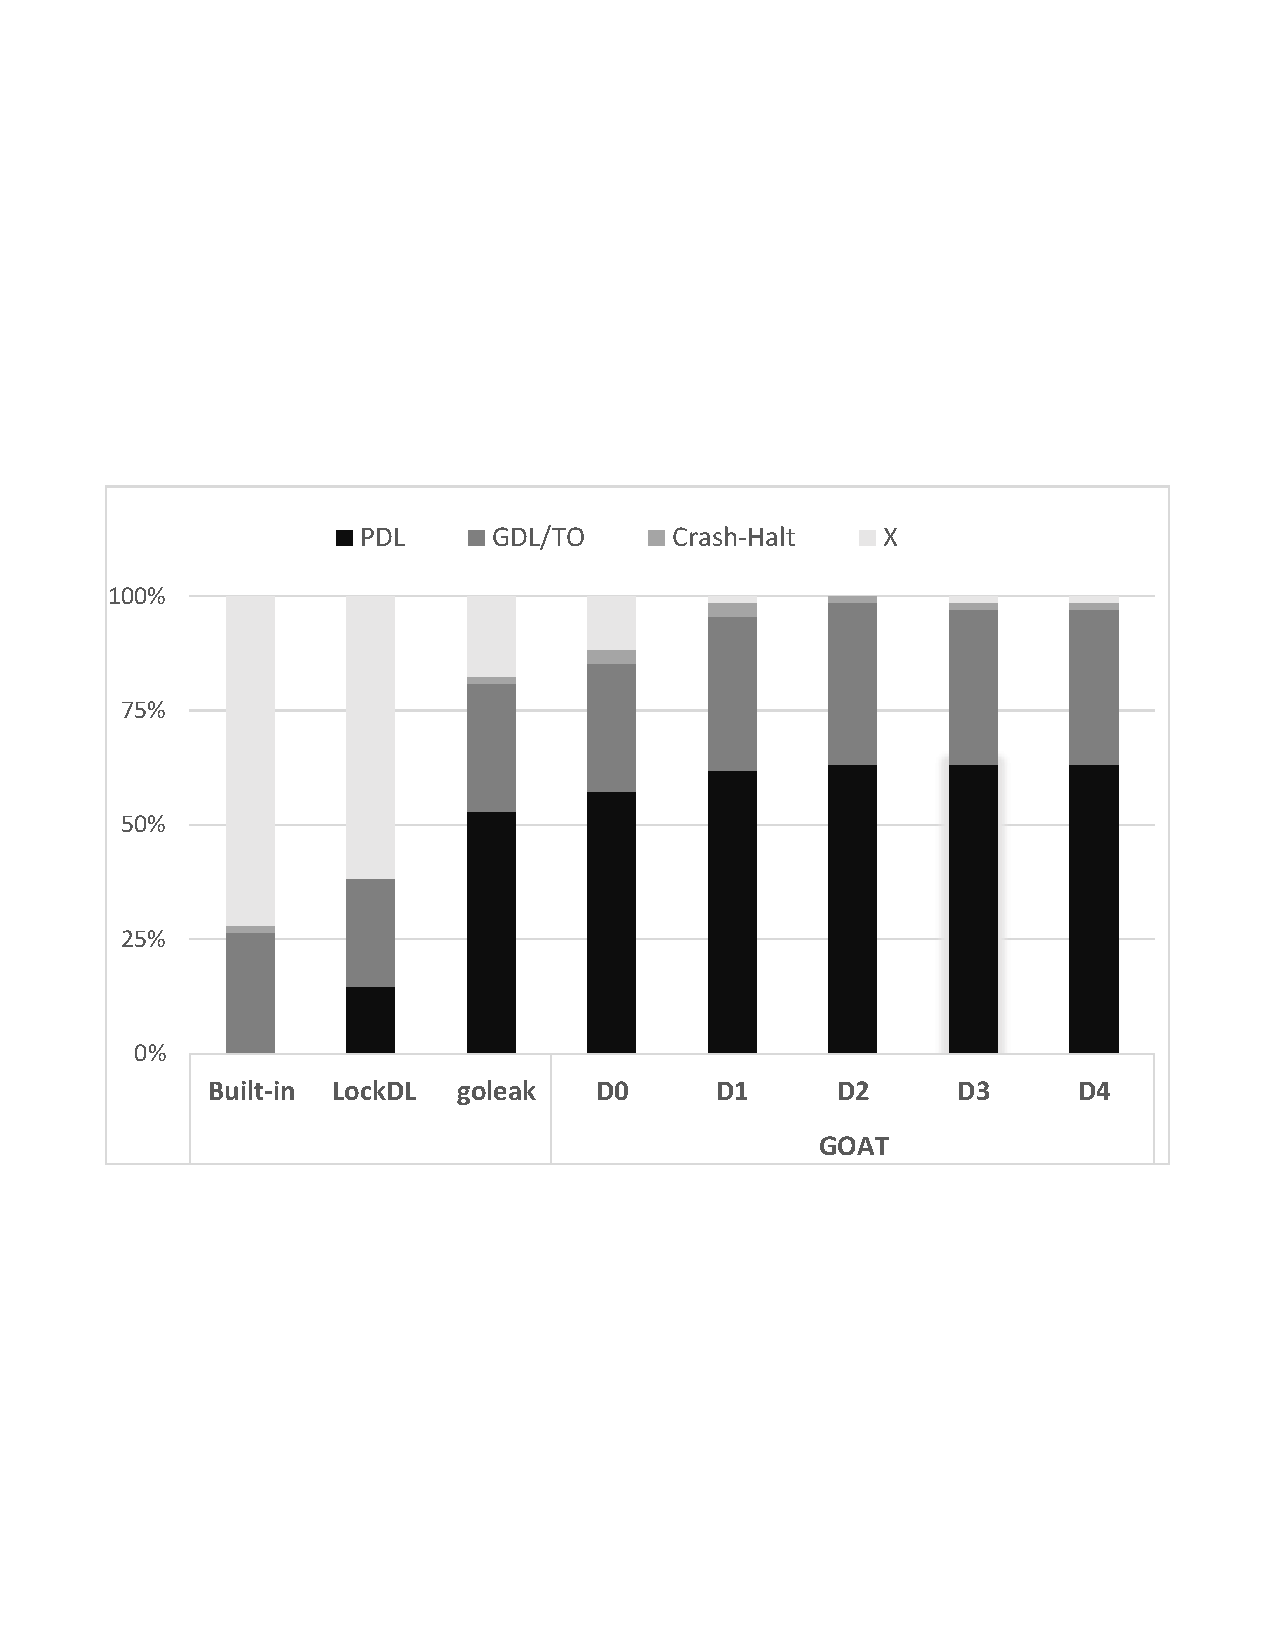
\includegraphics[width=.95\linewidth]{goat/figs/P4_detections.pdf}
  \caption{Histogram of detected bugs by each tool performed on 68 GoKer blocking bugs. PDL: partial deadlock, GDL/TO: global deadlock, Crash/Halt: causes the program to crash or halt during detection, X: nothing is detected }
  \label{fig:detection}
\end{minipage}
\begin{minipage}{.48\textwidth}
\centering
  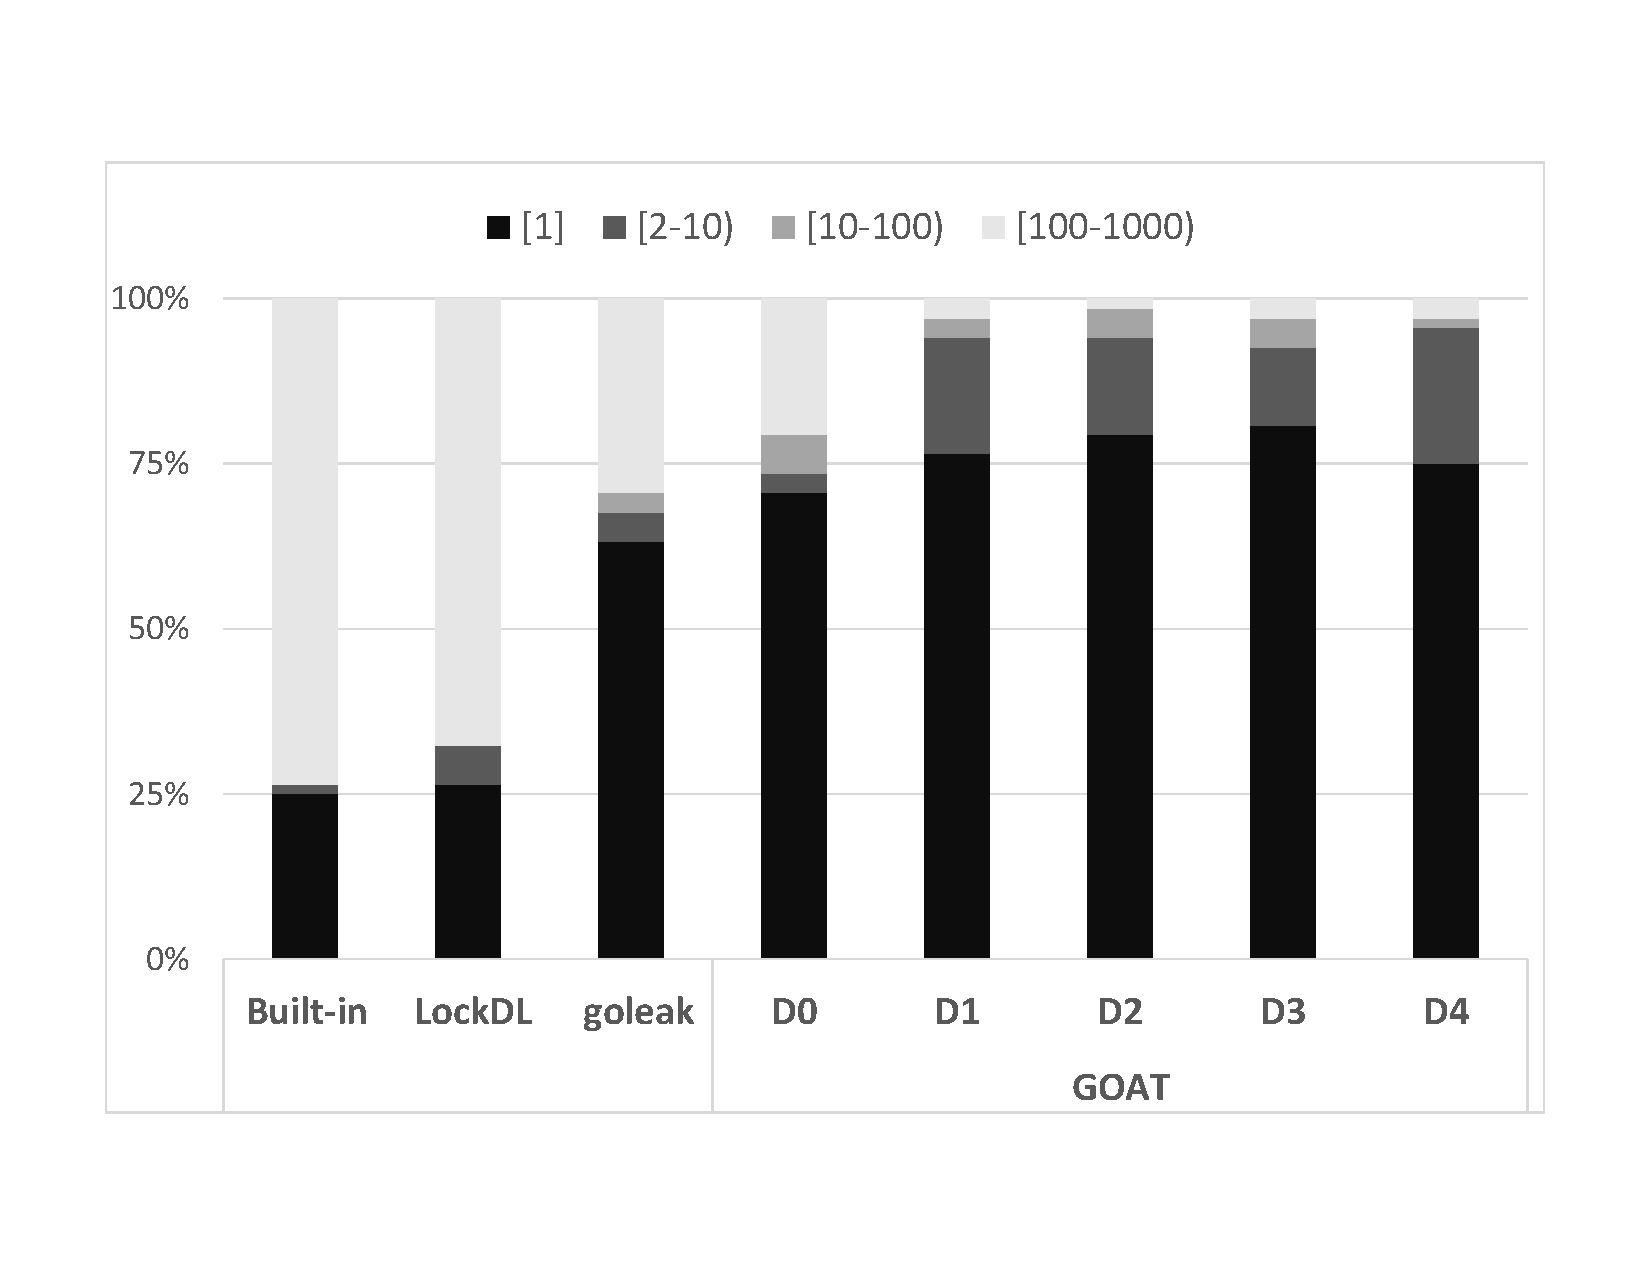
\includegraphics[width=.95\linewidth]{goat/figs/P4_runs.pdf}
  \caption{Histogram of required number of iterations by each tool to detect 68 GoKer blocking bugs}
  \label{fig:runs}
\end{minipage}
\end{figure}

\subsection{Deadlock Detection}
\label{sec:dl_evaluation}
We assess the ability of \goat and its variations in detecting bugs with minimum number of executions required to expose the bug.
%
We have compared \goat against three existing dynamic detectors:
\begin{itemize}
  \item \textit{Built-in} deadlock detector: It is an embeded mechanism in the standard Go runtime. The mechanism periodically makes sure that the queue of \textit{runnable} goroutines is never empty until the main goroutine terminates. If the queue is empty and main has not terminated yet (\ie main is blocked), it throws a runtime error.
  \item \textit{LockDL} \cite{lockdl}: This tool intercept with all mutex locks and unlocks of the target application to maintain a ``lock-set'' data structure. \textit{LockDL} issues warning during runtime when it finds a circular wait in the lock-set or double-locking the same lock. It has a timeout mechanism for application that traps into global deadlocks (30 seconds by default).
  \item \textit{goleak} \cite{goleak}: This leak detector from Uber checks the program stack at the end of the main goroutine's execution to find the application-level goroutines that remained in the stack (\ie leaked).
\end{itemize}

All experiments are performed on a server with two AMD Ryzen 5 3600 6-Core Processor (12 total cores with 2 threads per core and 6 cores per socket), 64 GB of RAM with generic Ubuntu 4.15.0 and Go version 1.15.6.
%
Table \ref{tab:comparison} shows the details of results obtained from executing each tool per bug 1000 times.
%
We show that the tool is unable to detect the bug after 1000 executions with \textbf{X (1000)}.
%

%
Figure \ref{fig:detection} and table \ref{tab:comparison} show that variations of \goat outperforms other detector by discovering the bug in 100\% of the GoKer blocking benchmark.
%
Figure \ref{fig:runs} and highlighted cells of table \ref{tab:comparison} show that the idea of injecting random delays around concurrency usage points in the program drastically reduces the required number of testing iterations until the bug occur.
%
D0 means \goat did not delay the program at any point and D4 means that the target program has been delayed up to four times around its CU points.
%
Figures \ref{fig:detection} and \ref{fig:runs} also state that the increase in the delay bound of \goat does not necessarily increase the chance of exposing the bug.
%
For example, the row of bug \texttt{serving\_2137} in table \ref{tab:comparison} show that only \goat D2 were able to detect the bug.


\begin{figure}[b]
\begin{minipage}{.48\textwidth}
\centering
  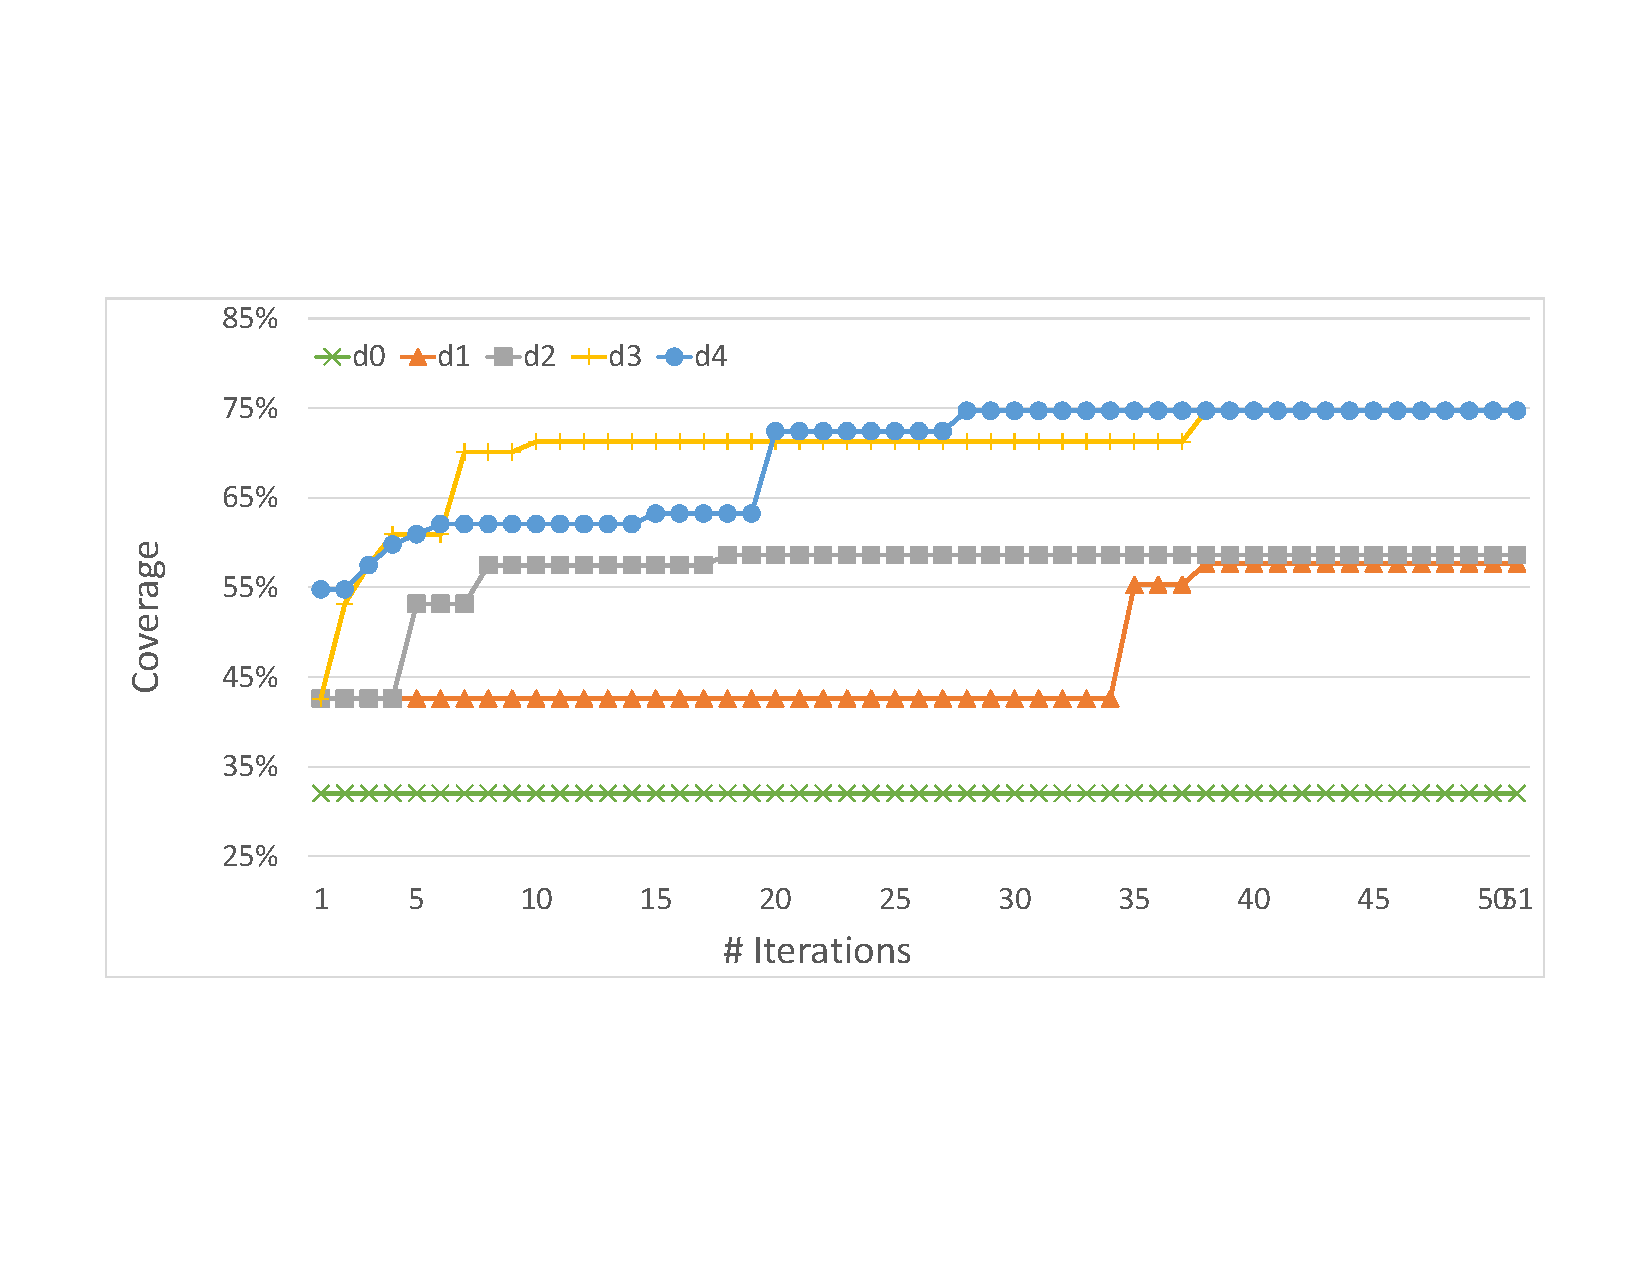
\includegraphics[width=.99\textwidth]{goat/figs/coverage_etcd7443.pdf}
  \caption{etcd7442 coverage}
  \label{fig:etcd_coverage}
\end{minipage}
\begin{minipage}{.48\textwidth}
\centering
  \includegraphics[width=.99\linewidth]{goat/figs/coverage_kubernetes11298.pdf}
  \caption{kuberenetes11298 coverage}
  \label{fig:kubernetes_coverage}
\end{minipage}
\end{figure}

\subsection{Coverage Analyis}
We picked two representative bug kernels \texttt{etcd7443} and \texttt{kubernetes11298} to evaluate the coverage idea on them as they
%
both have extensive use of channels, mutexes, conditional variables, nested selects within nested for loops and the buggy interleaving is proved to be rare to happen.
%
figures \ref{fig:etcd_coverage} and \ref{fig:kubernetes_coverage} show the gradual increase in coverage percentage during execution runs for different values of D.
%
Recall that D is the bound on the number of yields that we inject to the native execution of a given program to perturb the scheduler around concurrency usages.
%
These figures show that the increase of number of delays grows the rate of coverage percentage.
%
However, higher number of delays do not necessarily increase the coverage (D2 and D4 in figure \ref{fig:kubernetes_coverage}).
%
The drop in coverage for D1 in figure \ref{fig:kubernetes_coverage} is because of the new coverage requirements (\eg, a new goroutine is spawned and executing some concurrency primitives) that were encountered during testing execution.


%\section{GOAT: Coverage}
%\label{sec:coverage}
%
To demonstrate that testing has been thorough, \textit{coverage metrics} are defined to measure the progress of tests and specify testing termination condition.
%
Coverage metric for the set of testing executions $\mathcal{T}$ is a set of \textit{requirements} $\mathcal{R}$ that should get covered during testing iterations.
%
We say requirement $R_i$ is covered during testing iteration $t \in \mathcal{T}$ if we can correlate an \textit{action} during execution of $t$ to $R_i$.
%
For example, in \textit{statement coverage}, which is a widely-used metric in testing sequential software, $R$ is the set of source locations (file and line numbers) in the target program
%
$R_i$ is covered by test execution $t$ if the statement at location $R_i$ is executed in $t$.
%
The \textit{coverage percentage} of a test $\mathcal{T}$ is the ratio of the requirements covered by at least one execution over the number of all requirements ($|R|$).

As explained in Section \ref{sec:bg}, concurrent software testing frameworks perform testing iterations to explore the schedule-space and expose flaws.
%
Depending on the class of target bug, different coverage metrics are proposed and used for concurrent software testing.
%
\textit{Synchronization} coverage metrics such as \textit{blocking-blocked} \cite{edelstein2003contest}, \textit{blocked-pair-follows} \cite{trainin-followsCoverage-padtad09} and \textit{synchronization-pair} \cite{hong-syncTesting-issta12} defined requirements to cover during testing for exposing blocking bugs (\eg deadlocks).
%
%\textit{Memory access} coverage metrics such as PSet \cite{yu-pser-isca09} and def-use \cite{yang-defuse-issta98} focuses on data-access related bugs such as atomicity violation or data races.
%
For example, the synchronization coverage model in \cite{edelstein2003contest} defines \textit{blocking} and \textit{blocked} requirements per each synchronized block (\ie mutually exclusive section of the code that is protected by a lock).
%
The purpose of this requirement is to check if a test can report when there is a lock contention for two or more threads entering the synchronized block.
%
That is, a thread is either \textit{blocked} from entering the synchronization block or \textit{blocking} other threads from entering by holding the lock.
%

Proposed concurrency coverage metrics are mostly in the context of Java and C/Pthreads and are not directly applicable to languages like Go as Go has different concurrncy primitives and semantics.
%
Bron et. al,\cite{bron-appSyncCov-ppopp05} enumerates four major characteristics for coverage metrics to gain acceptance:
\begin{itemize}
  \item \textbf{Fixed model:} The metric should be well-understood by the developer or tester. A static model of requirements from target program should be constructed by instrumenting the source-code. The model should maintain covered requirements during testing executions.
  \item \textbf{Coverable and measurable requirements:} The absolute majority of reqiurements should be realistic enough to be \textit{coverable} during testing. For a few that are not coverable (due to program semantics) or not \textit{measurable} (because of technical limitations), the devloper should be aware of the reason.
  \item \textbf{Actions for uncovered requirements:} After testing terminates, every uncovered requirement should yield an action (\eg extending testing iterations or removing dead code from the program thus removing uncoverable requirements)
  \item \textbf{Coverage satisfaction:} Some action should be taken upon reaching a threshold of coverage percentage (e.g., testing phase termination when reaching 100\% statement coverage)
\end{itemize}

Defining a new coverage metric to satisfy above characteristics requires an accurate and proper mental model of target bugs.
%
Based on our observations from execution of Go applications and bug kernels on the behavior of concurrency primitives, we define a set of coverage requirements (summarized in Table \ref{tab:cov_req}):
%
\begin{itemize}
  \item \textbf{Req1 (Send/Recv):} \{\texttt{blocked}, \texttt{unblocking}, \texttt{NOP}\} -- Goroutine $G_1$ is either \textit{blocked} on a channel send (receive) if the receiver (sender) goroutine $G_2$ is not ready or \textit{unblocking} the waiting receiver (sender) goroutine $G_2$. A channel send or receive might also be neither blocked nor unblocking (NOP) for buffered channels.
  \item \textbf{Req2 (Select-Case):} \{\texttt{blocked}, \texttt{unblocking}, \texttt{NOP}\} $\times$ \{\texttt{case}$_i$\} -- cases of select statements are channel sends and recives (or default case for non-blocking selects). For all select statements that has no default case, we obtain the cases of each select statement at runtime and maintain an instance of Req1 per case.
  \item \textbf{Req3 (Lock):} \{\texttt{blocked}, \texttt{blocking}\} -- Goroutine $G_i$ is either \textit{blocked} when locking a mutex because another goroutine has locked the mutex or \textit{blocking} other goroutines from acquiring the mutex lock.
  \item \textbf{Req4 (Unblocking):} \{\texttt{unblocking}, \texttt{NOP}\} -- The goroutine that is performing channel close, mutex unlock, conditional variable signal and broadcast, waitGroup done and non-blocking select case (send or receive) has two kinds of behavior. They either \textit{unblock} one or more waiting goroutines or has no effect (NOP).
  \item \textbf{Req5-Go:} \{\texttt{NOP}\} -- We emit a NOP action for each goroutine creation to indicate that it is covered during testing.
\end{itemize}


These requirements are effective because with the help of \goat infrastructure, they satisfy the characteristics of an ``acceptable'' coverage metric:
\begin{itemize}
  \item A \textit{fixed concurrency model} from target application is statically obtained by identifying CU points.
  \item We can measure whether the requirement has been covered by analyzing the test ECT. By maintaining a global data structure during execution of all $t \in \mathcal{T}$, we can evaluate the coverability of proposed requirements
  \item Every uncovered requirement report something meaningful. For example, if a send is always performing as \textit{unblocking} and never as \textit{blocked}, which means that receiver of this send always performs receive before sender reaches its send statement. In other words, the receive action \textit{always happen-before} send action. Perhaps this pattern of communication is part of the program semantic and matches developer's expectations (e.g., a set of goroutines are listening on a channel to perform non-frequent requests). Otherwise, it reflects a bug or flaw in the program design.
  \item Since \goat is able to detect occured blocking bugs and also maintain a global coverage model during testing iterations, testing phase can terminate either by detection of a bug or reaching a coverage percentage threshold.
\end{itemize}

Table \ref{tab:moby_cov_table} shows a representation of covered requirements after a successful run (run \#1) and a leaky execution (run \#2) of the program in listing \ref{listing:moby28462.minipage}.
%
The highlighted cells of the table are the requirements that were not covered in the successful run \#1 but covered in run \#2 in which the bug has revealed.
%



\begin{table}[]
\centering
\caption{Coverge requirements defined for concurrent Go}
\scalebox{0.9}{
\begin{tabular}{|
>{\columncolor[HTML]{FFFFFF}}l |
>{\columncolor[HTML]{FFFFFF}}l |
>{\columncolor[HTML]{FFFFFF}}c |
>{\columncolor[HTML]{FFFFFF}}c |
>{\columncolor[HTML]{FFFFFF}}c |
>{\columncolor[HTML]{FFFFFF}}c |}
\hline
\multicolumn{1}{|c|}{\cellcolor[HTML]{FFFFFF}} & \multicolumn{1}{c|}{\cellcolor[HTML]{FFFFFF}} & \multicolumn{4}{c|}{\cellcolor[HTML]{FFFFFF}Coverage Requirement Types} \\ \cline{3-6}
\multicolumn{1}{|c|}{\multirow{-2}{*}{\cellcolor[HTML]{FFFFFF}\begin{tabular}[c]{@{}c@{}}Coverage\\ Requirements\end{tabular}}} & \multicolumn{1}{c|}{\multirow{-2}{*}{\cellcolor[HTML]{FFFFFF}\begin{tabular}[c]{@{}c@{}}Concurrent\\ Action\end{tabular}}} & Blocked & Unblocking & Blocking & NOP \\ \hline
\cellcolor[HTML]{FFFFFF} & SEND & * & * &  & * \\ \cline{2-6}
\multirow{-2}{*}{\cellcolor[HTML]{FFFFFF}Req. 1: Send/Recv} & RECV & * & * &  & * \\ \hline
\cellcolor[HTML]{FFFFFF} & CASE$_i$ (SEND) & * & * &  & * \\ \cline{2-6}
\multirow{-2}{*}{\cellcolor[HTML]{FFFFFF}Req. 2: Select-Case} & CASE$_i$ (RECV) & * & * &  & * \\ \hline
Req. 3: Lock & LOCK & * &  & * &  \\ \hline
\cellcolor[HTML]{FFFFFF} & CLOSE &  & * &  & * \\ \cline{2-6}
\cellcolor[HTML]{FFFFFF} & UNLOCK &  & * &  & * \\ \cline{2-6}
\cellcolor[HTML]{FFFFFF} & SIGNAL &  & * &  & * \\ \cline{2-6}
\cellcolor[HTML]{FFFFFF} & BRDCST &  & * &  & * \\ \cline{2-6}
\multirow{-5}{*}{\cellcolor[HTML]{FFFFFF}Req. 4: Unblocking} & NB-SELECT &  & * &  & * \\ \hline
Req. 5: Go & Go &  &  &  & * \\ \hline
\end{tabular}

}
\label{tab:cov_req}
\end{table}



%\textbf{Req5-Wait:} \{\texttt{blocked},\texttt{non-blocking}\} -- the goroutine that performs a conditional variable or waitGroup Wait is either blocked waiting for a wake-up signal from other goroutines or is non-blocking when

\begin{figure}
\centering
  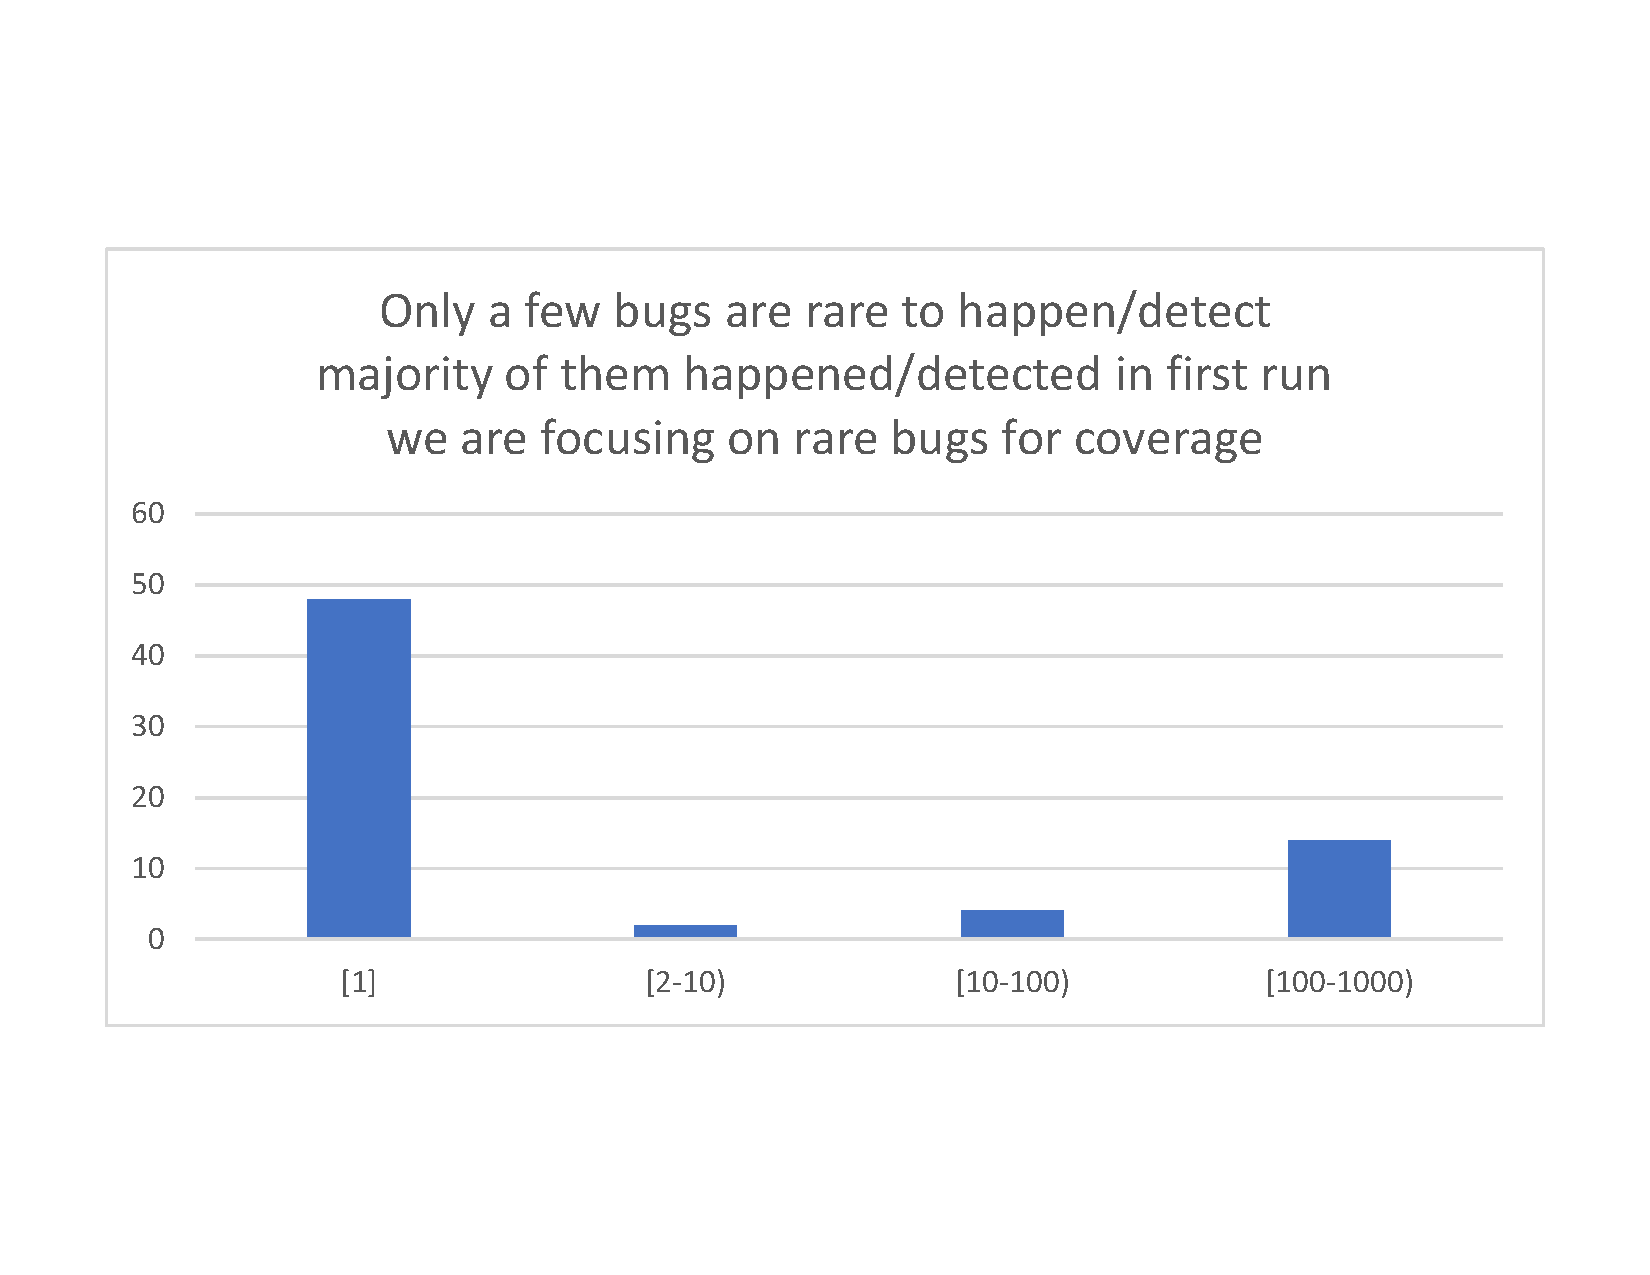
\includegraphics[width=.95\linewidth]{figs/coverage_motivation_tentative.pdf}
  \caption{focusing on rare bugs}
  \label{fig:rare_bugs}
\end{figure}



\subsection{Implementation}
Through a replay (\ie parsing the sequence) of ECT, a mapping between dynamic concurrent events and statically obtained CU points is emited by matching their respective call-stack and CU source location.
%
Through a BFS traversal of the goroutine tree, we add a \textit{coverage vector} to each goroutine node from the emitted mapping. Each element of the coverage vector is the respective covered value of requirement $R_i$ for the current goroutine node.
%
During executions of tests $t \in \mathcal{T}$, we maintain and update a global goroutine tree after each $t$.
%
It is crucial to maintain a global goroutine tree to measure the progress of coverage percentage over tests in $\mathcal{T}$.
%
Two goroutines $G_m$ and $G_n$ in the tests $t_i$ and $t_j$ are \textit{equivalent} (\ie falls into identical node in the global goroutine tree) if their parents are equivalent and their creation source location (CU of kind \texttt{go}) are identical:
\begin{equation}
  G_m \equiv G_n   \text{if}
  \begin{cases}
    \text{parent}(G_m) \equiv \text{parent}(G_n)  \wedge \\
    \text{CU(}G_m\text{).file} = \text{CU(}G_n\text{).file}  \wedge\\
    \text{CU(}G_m\text{).line} = \text{CU(}G_n\text{).line} \\
  \end{cases}
\end{equation}





\subsection{Evaluation}
We picked two representative bug kernels \texttt{etcd7443} and \texttt{kubernetes11298} to evaluate the coverage idea on them as they
%
They both have extensive use of channels, mutexes, conditional variables, nested selects within nested for loops and the buggy interleaving is proved to be rare to happen.
%
figures \ref{etcd_coverage} and \ref{fig:kubernetes_coverage} show the gradual increase in coverage percentage during execution runs for different values of D.
%
Recall that D is the bound on the number of yields that we inject to the native execution of a given program to perturb the scheduler around concurrency usages.
%
These figures show that
%


\begin{figure}
\centering
  \includegraphics[width=.95\linewidth]{figs/coverage_kubernetes11298.pdf}
  \caption{kuberenetes11298 coverage}
  \label{fig:kubernetes_coverage}
\end{figure}



\section{Related Work}
\label{sec:ch4_related}
\subsection{Go Correctness}
Decades of research effort have been dedicated to the logical and performance correctness of concurrent and parallel programs.
%
For CSP-based concurrent languages like Go, static (source-level) analysis methods \cite{ng-dl-cc16,lange-fence-popl17,lange-staticType-icse18} tend to assure bug freedom and verify safety properties through abstractions like session types and choreography synthesis.
%
Ng and Yoshida \cite{ng-dl-cc16} first proposed a static tool to detect global deadlock in Go programs using choreography synthesis.
%
Later, Stadtmuller et al. \cite{stadtmuller-minigo-aplas16} proposed a static trace-based global detection approach based on forkable regular expressions.
%
Lange et al. proposed more static verification frameworks for checking channel safety, and liveness \cite{lange-fence-popl17}, and behavioral model checking \cite{lange-staticType-icse18}.
%
Both methods approximate Go programs with session types and behavioral contracts extracted from their SSA intermediate representation.
%
The mentioned work has limitations for handling dynamic (e.g., in-loop) goroutine or channel creation.
%
They also do not scale and are impractical in real-world programs due to the state explosion problem and lack of proper front-end interface \cite{yuan-gobench-cgo21}.
%
Besides, similar to other static analysis methods, they often suffer from false positives due to conservative constraints.

%
Dynamic (runtime-level) analysis approaches \cite{sulzmann-twophase-2018,dilley-gomela-corr2020} rely on code instrumentation and program rewrites to obtain and analyze an \textit{execution model}.
%
Zhao et al. \cite{zhao-occam97} introduced a runtime monitoring approach for deadlock detection for Occam programs based on wait-for graphs and some heuristics. Occam is a concurrent language based on CSP semantics, and similar to Go, it uses channels to establish communication between processes.
%
Sulzmann and Stadtmuller proposed a dynamic verification approach for synchronous (unbuffered) channels \cite{sulzmann-corr17}, and a vector-clock-based approach for asynchronous channels \cite{sulzmann-twophase-2018}.
%
Although they may support a larger subset of the Go language, they only focus on channels as the root cause of deadlocks and evaluated only on relatively small examples.
%
Also, they usually do not scale for real-world Go applications with thousands of goroutines and LOC \cite{dilley-empirical-saner19}.
%

Standard Go comes with a few dynamic analysis tools. For example, the \textit{race detector} \cite{go-race-blog} which is basically a wrapper around ThreadSanitizer \cite{konstantin-tsan-wbia09}, tracks memory accesses and detect races that happened during execution.
%
A few other facilities for code coverage measurement, profiling, and tracing \cite{go-package-trace} are provided to deliver insight into the testing quality and performance behavior.
%
The built-in race detector \cite{go-race-blog}, despite its limitations (\eg, supporting up to 8192 goroutines), has proved to be effective in dynamically detecting data races in most cases quickly.

\subsection{Systematic Testing}
Systematic testing combines ideas from static and dynamic approaches to reduce the state space and reflect realistic behavior.
%
Assuming the scheduler causes concurrency bugs (and not the program input), they may not manifest during conventional testing and difficult to reproduce, both due to nondeterministic decisions that the scheduler makes.
%
Researchers have applied different methods \cite{thomson-concurrencyTesting-ppopp14} to reduce the interleaving space to explore effectively and efficiently.
%
Delay-bounded \cite{emmi-delayBounded-popl11,burckhardt-depthBug-asplos10} and preemption-bounded \cite{madanlal-preemptionBound-pldi07} techniques systematically ``fuzz'' the scheduler to equally and fairly cover feasible interleaving.
%
Other tools like Maple \cite{yu-maple-oopsla12}, CalFuzzer \cite{joshi-calfuzzer},  and ConTest \cite{contest-jgi01,edelstein2003contest} \textit{actively} control the scheduler to maximise a predefined concurrency coverage criterion \cite{hong-syncTesting-issta12} or the probability of bug exposure \cite{burckhardt-depthBug-asplos10}.



\section{Summary \& Future Work}
\label{sec:ch4_summary}
We presented \goat, an analysis and testing framework for concurrent Go applications to assist concurrency debugging of real-world applications.
%
\goat combines static and dynamic methods to model and explore application execution.
%
The scheduler behavior is pertubed with automatically injected random delays to accelerate the exposure of bug, if any.
%
By dynamic measurment of a set of coverage requirements, we quantify the quality of schedule-space exploration of \goat.
%
\goat detects all 68 blocking bugs of GoKer benchmark which are the bug kernels of top nine open-soruce projects written in Go.
%
The schedule perturbation showed effectiveness in accelerating the bug exposure.
%
Proposed coverage requirements accurately reflect the dynamic behavior of program executions and testing iterations.

Engineering of \goat is flexible and extensible to more advanced components.
%
For example, current minimal \goat engine can be extended to take the full control over the Go scheduler and ``guide'' testing towards untested interleaving.
%
We are dockerizing \goat for easy and public use.
%
We want to test on real-world programs.
%
The data that ECT includes is rich enough for training accurate models and apply machine learning methods to learn and predict bug patterns.

